\documentclass[12pt,a4paper]{article}
\usepackage[utf8]{inputenc}
\usepackage[spanish]{babel}
\usepackage{graphicx}
\usepackage{subcaption}
\usepackage{float}
\usepackage{listings}
\usepackage{xcolor}
\usepackage{hyperref}
\usepackage{geometry}
\geometry{top=2.5cm, bottom=2.5cm, left=3cm, right=3cm}
\graphicspath{{Imagenes/}}
% Colores para los codigos parecidos a MySQL
\definecolor{codegreen}{rgb}{0,0.6,0}
\definecolor{codegray}{rgb}{0.5,0.5,0.5}
\definecolor{codepurple}{rgb}{0.58,0,0.82}
\definecolor{backcolour}{rgb}{0.95,0.95,0.92}

\lstset{
    language=SQL,
    backgroundcolor=\color{backcolour},   
    commentstyle=\color{codegreen},
    keywordstyle=\color{blue}\bfseries,
    numberstyle=\tiny\color{codegray},
    stringstyle=\color{codepurple},
    basicstyle=\ttfamily\scriptsize,
    breakatwhitespace=false,         
    breaklines=true,                 
    captionpos=b,                    
    keepspaces=true,                 
    showspaces=false,                
    showstringspaces=false,
    showtabs=false,                  
    tabsize=4,
    frame=single
}

\begin{document}
\begin{titlepage}
    \centering
    \vspace*{2cm}
    
    \Huge
    \textbf{Proyecto de Bases de Datos}
    
    \vspace{0.5cm}
    \LARGE
    Sistema de gestión de tienda online
    
    \vspace{2cm}
    \textbf{Materia:} Bases de Datos
    
    \vspace{1cm}
    \textbf{Alumno:} Alexandra Jokebed Hernandez Garcilitas 
    
    \vspace{1cm}
    \textbf{Profesor:} Dr. Guillermo Monroy Rodriguez 
    
    \vfill
    
    \Large
    \today
\end{titlepage}


\newpage
\tableofcontents
\newpage


\section{Análisis y diseño}

\subsection{Modelo conceptual y Diagrama Entidad-Relación (DER)}
Previo a la implementación física en el Sistema Gestor de Bases de Datos (SGBD), en este caso MySQL, se realizó un análisis de los requerimientos de la tienda online para modelar las entidades, atributos y restricciones del negocio. El primer paso consistió en la elaboración de un diagrama conceptual que mapea las 6 entidades fundamentales del sistema y sus relaciones cardinales.

\begin{figure}[H]
    \centering
    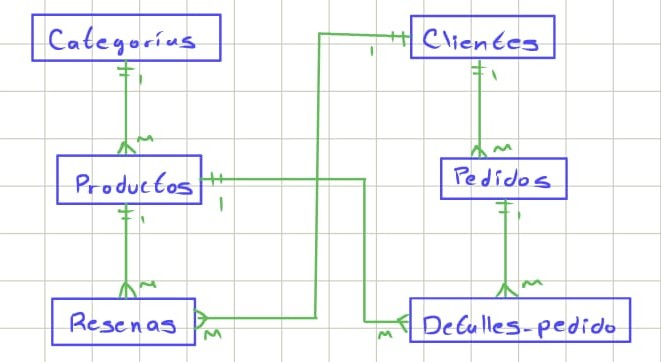
\includegraphics[width=0.55\textwidth]{ADDER.jpeg}
    \caption{Definición de entidades y atributos.}
\end{figure}

\begin{figure}[H]
    \centering
    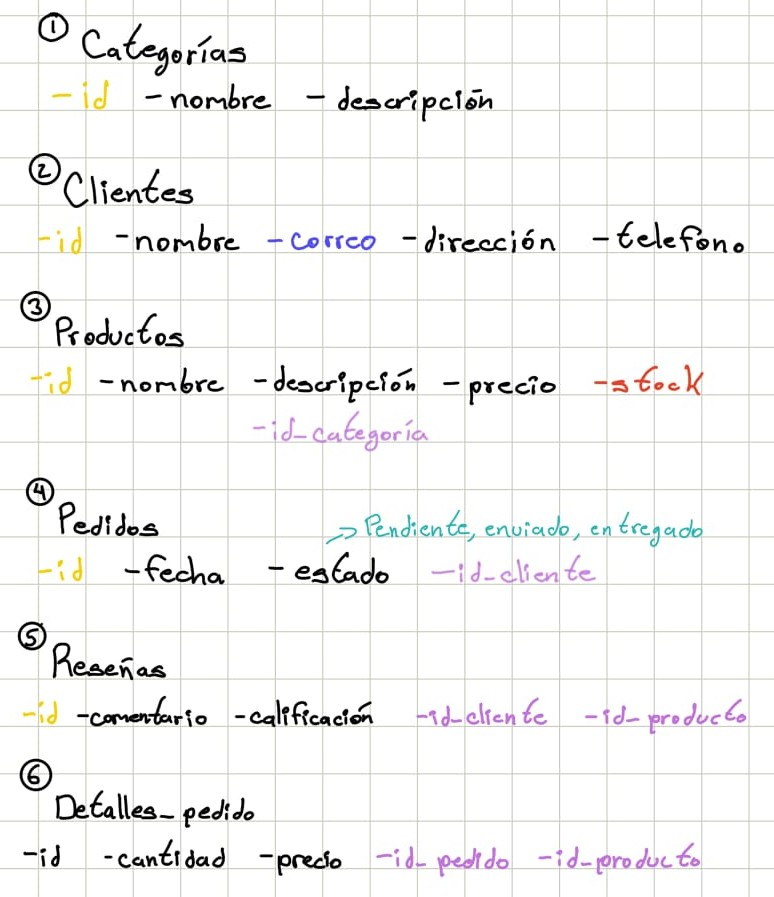
\includegraphics[width=0.55\textwidth]{ADT.jpeg}
    \caption{Borrador conceptual del Modelo Entidad-Relación.}
\end{figure}

En este diseño preliminar se establecieron las bases de la integridad referencial mediante un código de diseño visual:
\begin{itemize}
    \item \textbf{Identificadores únicos (Claves Primarias):} Marcados en amarillo (id), garantizando que cada registro sea irrepetible.
    \item \textbf{Relaciones (Claves Foráneas):} Marcadas en morado (id\_categoria, id\_cliente, etc.), las cuales construyen la navegación relacional entre las entidades.
    \item \textbf{Restricciones de Negocio:} Se identificaron reglas críticas, como la unicidad del correo electrónico (azul) y la restricción para que el stock no asuma valores negativos (rojo). Se delimitó el dominio del estado del pedido (pendiente, enviado, entregado).
\end{itemize}

Para complementar el análisis, a continuación se presenta el diagrama generado mediante ingeniería inversa, reflejando el esquema final implementado.

\begin{figure}[H]
    \centering
    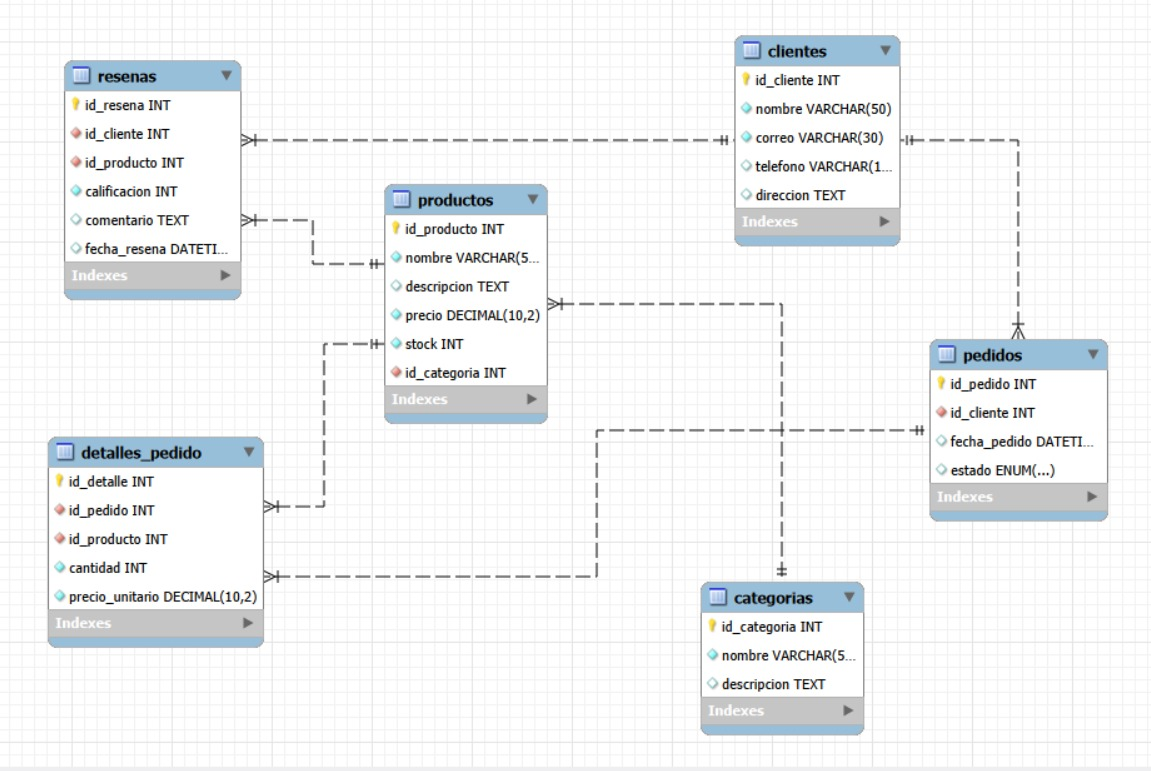
\includegraphics[width=1\textwidth]{DER.jpeg}
    \caption{Diagrama Entidad-Relación generado mediante ingeniería inversa (MySQL Workbench).}
\end{figure}

\subsection{Justificación de la Normalización (3NF)}
El esquema cumple con las reglas de la Tercera Forma Normal (3NF) justificado por las siguientes decisiones:
\begin{itemize}
    \item \textbf{Primera Forma Normal (1NF) - Atomicidad:} Todos los atributos contienen valores atómicos. La dirección y el teléfono del cliente están separados y almacenan un solo valor por columna.
    \item \textbf{Segunda Forma Normal (2NF) - Dependencia completa:} Todos los atributos no clave dependen de la clave primaria. Para relaciones de muchos a muchos (N:M), se implementaron tablas intermedias (ej. \texttt{detalles\_pedido}), la cual absorbe las claves foráneas y guarda la cantidad y precio exacto al momento de la transacción.
    \item \textbf{Tercera Forma Normal (3NF) - Sin dependencias transitivas:} Ningún atributo no clave depende de otro. Se aisló la entidad \texttt{categorias} y se vinculó mediante \texttt{id\_categoria} en los productos, evitando redundancia de nombres. Las \texttt{resenas} dependen directamente del cruce cliente-producto.
\end{itemize}


\section{Implementación de la Base de Datos}

\subsection{Creación de la BD y Tablas}
\begin{lstlisting}
DROP DATABASE IF EXISTS tienda_online; -- Limpiamos la base de datos por si nos hemos equivocado anteriormente
CREATE DATABASE tienda_online;
USE tienda_online;

-- Creamos la tabla de categorias
CREATE TABLE categorias (
    id_categoria INT AUTO_INCREMENT NOT NULL PRIMARY KEY,
    nombre VARCHAR(50) NOT NULL,
    descripcion TEXT
);

-- Creamos la tabla de clientes 
CREATE TABLE clientes (
    id_cliente INT AUTO_INCREMENT NOT NULL PRIMARY KEY,
    nombre VARCHAR(50) NOT NULL,
    correo VARCHAR(30) NOT NULL UNIQUE, -- Ponemos UNIQUE para que no puedan exitir varios registros con el mismo correo
    telefono VARCHAR(10),
    direccion TEXT
);

-- Creaos la tabla de los productos
CREATE TABLE productos (
    id_producto INT AUTO_INCREMENT NOT NULL PRIMARY KEY,
    nombre VARCHAR(50) NOT NULL,
    descripcion TEXT,
    precio DECIMAL(10,2) NOT NULL,
    stock INT NOT NULL CHECK (stock >= 0), -- Establecemos que el stock debe ser igual o mayor a 0, esto para evitar que sea negativo
    id_categoria INT NOT NULL,
    FOREIGN KEY (id_categoria) REFERENCES categorias(id_categoria) -- Esto funciona como puente donde decimos que los valores de la columna id_categoria en esta tabla (FK) dependen del id_categoria de la tabla de categorias
);

-- Creamos la tabla de pedidos
CREATE TABLE pedidos (
    id_pedido INT AUTO_INCREMENT NOT NULL PRIMARY KEY,
    id_cliente INT NOT NULL,
    fecha_pedido DATETIME DEFAULT CURRENT_TIMESTAMP,
    estado ENUM('pendiente', 'enviado', 'entregado') DEFAULT 'pendiente', -- ENUM nos sirve para poner una restrccion de que en la columna "estado" solo aceptamos las palabras senaladas entre parentesis
    FOREIGN KEY (id_cliente) REFERENCES clientes(id_cliente) -- Establecemos que cada pedido tendra un identificador del cliente que lo pidio como una FK, esto depende del id del cleinte en la tabla de clientes
);

-- Creamos la tabla para especificar los detalles de cada pedido 
CREATE TABLE detalles_pedido (
    id_detalle INT AUTO_INCREMENT NOT NULL PRIMARY KEY,
    id_pedido INT NOT NULL,
    id_producto INT NOT NULL,
    cantidad INT NOT NULL,
    precio_unitario DECIMAL(10,2) NOT NULL,
    FOREIGN KEY (id_pedido) REFERENCES pedidos(id_pedido) ON DELETE CASCADE, -- Establecemos el puente de la FK del id de los pedidos con la tabla pedidos, ademas agregamos la condicion de "ON DELETE CASCADE" para que en caso de que borren cualquier pedido se borre tambien cualquier detalle sobre dicho pedido de manera automatica y nos ahorra el trabajo manual
    FOREIGN KEY (id_producto) REFERENCES productos(id_producto)
);

-- Creamos la tabla para las resenas de los clientes
CREATE TABLE resenas (
    id_resena INT AUTO_INCREMENT NOT NULL PRIMARY KEY,
    id_cliente INT NOT NULL,
    id_producto INT NOT NULL,
    calificacion INT NOT NULL CHECK (calificacion BETWEEN 1 AND 5), -- Decimos que aqui solamente se aceptan valores desde el 1 al 5 incluyendo a dichos numeros
    comentario TEXT,
    fecha_resena DATETIME DEFAULT CURRENT_TIMESTAMP,
    FOREIGN KEY (id_cliente) REFERENCES clientes(id_cliente),
    FOREIGN KEY (id_producto) REFERENCES productos(id_producto)
);
\end{lstlisting}
\begin{figure}[H]
    \centering
    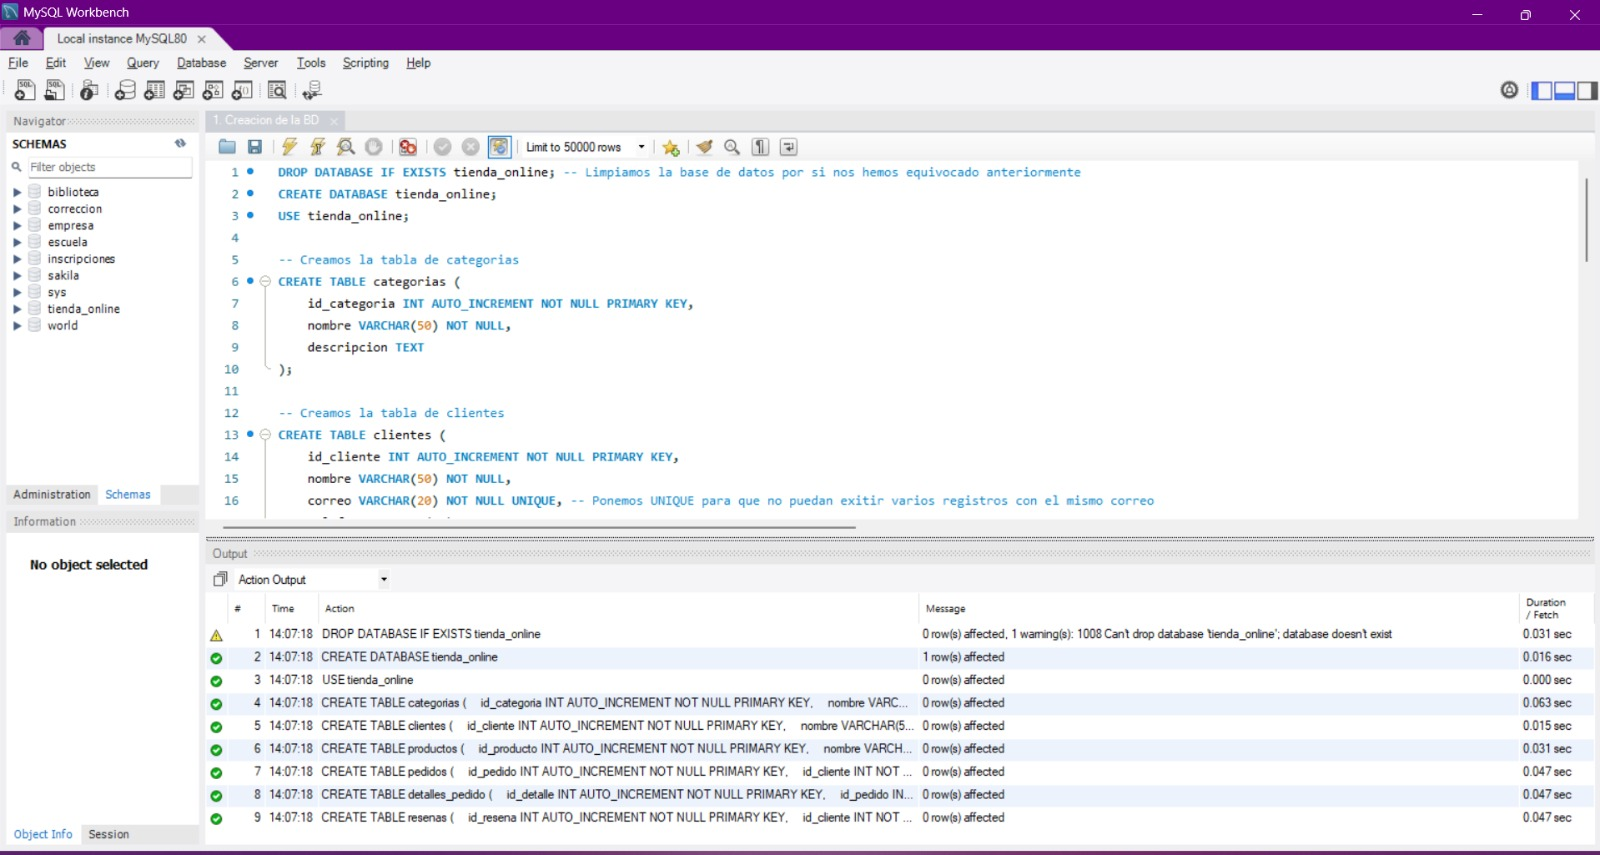
\includegraphics[width=0.9\textwidth]{CBD.jpeg}
    \caption{Ejecución exitosa de la creación de la base de datos.}
\end{figure}

\subsection{Llenado de la base de datos}
\begin{lstlisting}
USE tienda_online;

-- Insertamos 5 datos para la tabla categorias
INSERT INTO categorias (nombre, descripcion) VALUES 
('Smartphones', 'Telefonos moviles de ultima generacion'),
('Laptops', 'Computadoras portatiles para trabajo y gaming'),
('Wearables', 'Relojes inteligentes y pulseras de actividad'),
('Audio', 'Audifonos, bocinas y equipos de sonido'),
('Accesorios', 'Cables, fundas, cargadores y mouses');

-- Insertamos los datos de 15 clientes
INSERT INTO clientes (nombre, correo, telefono, direccion) VALUES 
('Carlos Mendoza', 'carlos.m@cua.uam.mx', '5551234567', 'Av. Vasco de Quiroga 4871'),
('Ana Sofia Lopez', 'ana.lopez@gmail.com', '5559876543', 'Col. Santa Fe, CDMX'),
('Luis Perez', 'luis.perez@hotmail.com', '5551112233', 'Av. Constituyentes 100'),
('Maria Garcia', 'maria.g@yahoo.com', '5554445566', 'Calle 10, Cuajimalpa'),
('Javier Hernandez', 'javier.h@gmail.com', '5557778899', 'Bosques de las Lomas'),
('Laura Martinez', 'laura.m@outlook.com', '5550001122', 'Interlomas, Huixquilucan'),
('Roberto Gomez', 'roberto.g@gmail.com', '5553334455', 'Polanco, CDMX'),
('Diana Torres', 'diana.t@cua.uam.mx', '5556667788', 'Contadero, Cuajimalpa'),
('Fernando Ruiz', 'fernando.r@hotmail.com', '5559990011', 'Condesa, CDMX'),
('Carmen Silva', 'carmen.s@gmail.com', '5552223344', 'Roma Norte, CDMX'),
('Alejandro Vega', 'alejandro.v@yahoo.com', '5555556677', 'Del Valle, CDMX'),
('Patricia Castro', 'patricia.c@outlook.com', '5558889900', 'Narvarte, CDMX'),
('Ricardo Ortiz', 'ricardo.o@gmail.com', '5551239876', 'Coyoacan, CDMX'),
('Gabriela Navarro', 'gabriela.n@cua.uam.mx', '5554561239', 'San Angel, CDMX'),
('Hugo Morales', 'hugo.m@hotmail.com', '5557894561', 'Tlalpan, CDMX');

-- Insertamos 30 productos
INSERT INTO productos (nombre, descripcion, precio, stock, id_categoria) VALUES 
('iPhone 15 Pro', '256GB, Titanio', 23999.00, 15, 1),
('Samsung Galaxy S24 Ultra', '512GB, IA integrada', 25999.00, 10, 1),
('Google Pixel 8', '128GB, Android Puro', 15499.00, 8, 1),
('Xiaomi 14', '256GB, Carga ultrarrapida', 18999.00, 20, 1),
('Motorola Edge 40', '256GB, Pantalla curva', 11999.00, 25, 1),
('MacBook Pro M3', '14 pulgadas, 16GB RAM', 34999.00, 5, 2),
('Dell XPS 15', 'Intel Core i9, 32GB RAM', 38500.00, 4, 2),
('Asus ROG Zephyrus', 'RTX 4070, 16GB RAM', 32999.00, 7, 2),
('Lenovo ThinkPad X1', 'Core i7, Ultraligera', 28999.00, 12, 2),
('HP Spectre x360', 'Convertible, 16GB RAM', 27500.00, 9, 2),
('Acer Swift 3', 'Core i5, 8GB RAM', 14500.00, 15, 2),
('Apple Watch Series 9', '41mm, Aluminio', 8999.00, 30, 3),
('Samsung Galaxy Watch 6', '44mm, Bluetooth', 5499.00, 22, 3),
('Garmin Forerunner 265', 'Reloj GPS para correr', 9500.00, 10, 3),
('Amazfit GTR 4', 'Bateria de 14 daas', 3499.00, 40, 3),
('Fitbit Charge 6', 'Pulsera de actividad avanzada', 3199.00, 35, 3),
('AirPods Pro 2', 'Cancelacion de ruido activa', 5299.00, 50, 4),
('Sony WH-1000XM5', 'Diadema con noise cancelling', 6999.00, 18, 4),
('Bose QuietComfort Earbuds', 'In-ear premium', 5999.00, 12, 4),
('JBL Flip 6', 'Bocina Bluetooth resistente al agua', 2499.00, 45, 4),
('Samsung Galaxy Buds 2 Pro', 'Audio 360', 3899.00, 25, 4),
('Sennheiser Momentum 4', 'Bateria de 60 horas', 7499.00, 8, 4),
('Logitech MX Master 3S', 'Mouse ergonomico', 2199.00, 30, 5),
('Cargador Anker Nano II', '65W, USB-C', 899.00, 60, 5),
('Cable Apple USB-C', 'Trenzado, 2 metros', 599.00, 100, 5),
('Funda Spigen iPhone 15', 'Transparente anti-amarillo', 450.00, 55, 5),
('Mochila Targus', 'Para laptop 15.6 pulgadas', 950.00, 20, 5),
('Teclado Keychron K2', 'Mecanico inalambrico', 2100.00, 15, 5),
('Hub UGREEN USB-C', '7 en 1 con HDMI', 750.00, 40, 5),
('Base de carga Belkin', 'Inalambrica 3 en 1', 2500.00, 10, 5);

-- Insertamos 20 pedidos para diferentes clientes
INSERT INTO pedidos (id_cliente, estado) VALUES 
(1, 'entregado'), 
(2, 'enviado'), 
(3, 'pendiente'), 
(4, 'entregado'), 
(5, 'pendiente'),
(1, 'pendiente'), 
(6, 'enviado'), 
(7, 'entregado'), 
(8, 'pendiente'), 
(9, 'entregado'),
(10, 'pendiente'), 
(11, 'enviado'), 
(12, 'entregado'), 
(13, 'pendiente'), 
(14, 'entregado'),
(15, 'pendiente'), 
(2, 'entregado'), 
(3, 'enviado'), 
(4, 'pendiente'), 
(5, 'entregado');

-- Insertamos los detalles de cada pedido
INSERT INTO detalles_pedido (id_pedido, id_producto, cantidad, precio_unitario) VALUES 
(1, 1, 1, 23999.00), (1, 26, 1, 450.00),  -- Cliente 1 compra iPhone y funda
(2, 6, 1, 34999.00),                       -- Cliente 2 compra MacBook
(3, 17, 1, 5299.00), (3, 25, 2, 599.00),  -- Cliente 3 compra AirPods y 2 cables
(4, 23, 1, 2199.00),                       -- Cliente 4 compra Mouse
(5, 12, 1, 8999.00),                       -- Cliente 5 compra Apple Watch
(6, 20, 2, 2499.00),                       -- Cliente 1 compra 2 bocinas JBL
(7, 2, 1, 25999.00),                       -- Cliente 6 compra Samsung Ultra
(8, 7, 1, 38500.00), (8, 27, 1, 950.00),  -- Cliente 7 compra Dell XPS y mochila
(9, 13, 1, 5499.00),                       -- Cliente 8 compra Galaxy Watch
(10, 18, 1, 6999.00),                      -- Cliente 9 compra Sony WH
(11, 3, 1, 15499.00),                      -- Cliente 10 compra Pixel 8
(12, 28, 1, 2100.00),                      -- Cliente 11 compra Teclado
(13, 8, 1, 32999.00),                      -- Cliente 12 compra Asus ROG
(14, 21, 1, 3899.00), (14, 24, 1, 899.00),-- Cliente 13 compra Galaxy Buds y cargador
(15, 4, 1, 18999.00),                      -- Cliente 14 compra Xiaomi 14
(16, 29, 1, 750.00),                       -- Cliente 15 compra Hub
(17, 19, 1, 5999.00),                      -- Cliente 2 compra Bose
(18, 5, 1, 11999.00),                      -- Cliente 3 compra Motorola
(19, 10, 1, 27500.00),                     -- Cliente 4 compra HP Spectre
(20, 14, 1, 9500.00), (20, 30, 1, 2500.00);-- Cliente 5 compra Garmin y Base de carga

-- Insrtamos las resenas de cada cliente que YA haya comprado el producto 
INSERT INTO resenas (id_cliente, id_producto, calificacion, comentario) VALUES 
(1, 1, 5, 'Excelente telefono, la camara es increible y la bateria dura todo el dia.'),
(1, 26, 4, 'Buena funda, protege bien pero se raya un poco.'),
(2, 6, 5, 'La mejor laptop que he tenido, sUper rapida para programar.'),
(4, 23, 5, 'Super comodo para trabajar largas horas.'),
(7, 7, 4, 'Muy potente, pero se calienta un poco al jugar.'),
(7, 27, 5, 'Muy espaciosa y los materiales se sienten premium.'),
(9, 18, 5, 'La cancelacion de ruido es brutal, 100% recomendados.'),
(12, 8, 5, 'Corre todos los juegos en ultra sin problemas.'),
(14, 4, 4, 'Carga rapidisimo, buen equipo por el precio.'),
(2, 19, 3, 'Suenan bien, pero a veces se desconecta el bluetooth.');
\end{lstlisting}
\begin{figure}[H]
    \centering
    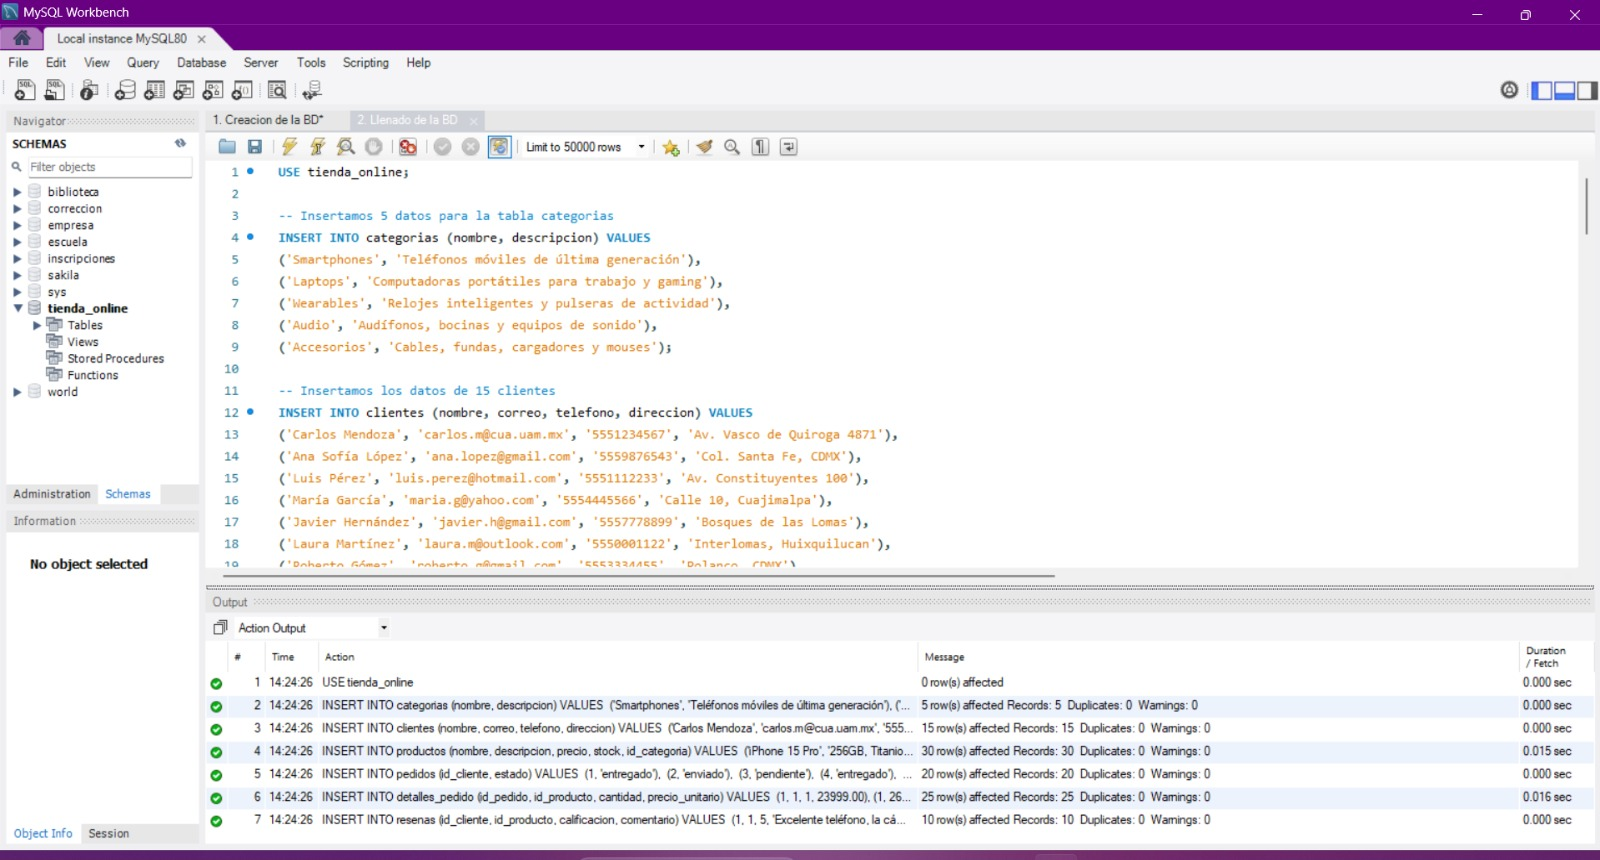
\includegraphics[width=0.9\textwidth]{LLBD.jpeg}
    \caption{Llenado de datos de prueba.}
\end{figure}


\section{Consultas SQL}

\subsection{Consulta 1: Productos disponibles por categoría}
\begin{lstlisting}
USE tienda_online;

-- Mostrar los productos disponibles y ordenarlos de acuerdo a su precio
SELECT c.nombre AS categoria, p.nombre AS producto, p.precio, p.stock
FROM productos p
JOIN categorias c ON p.id_categoria = c.id_categoria
WHERE p.stock > 0
ORDER BY c.nombre ASC, p.precio ASC;
\end{lstlisting}
\begin{figure}[H]
    \centering
    \begin{subfigure}{0.48\textwidth}
        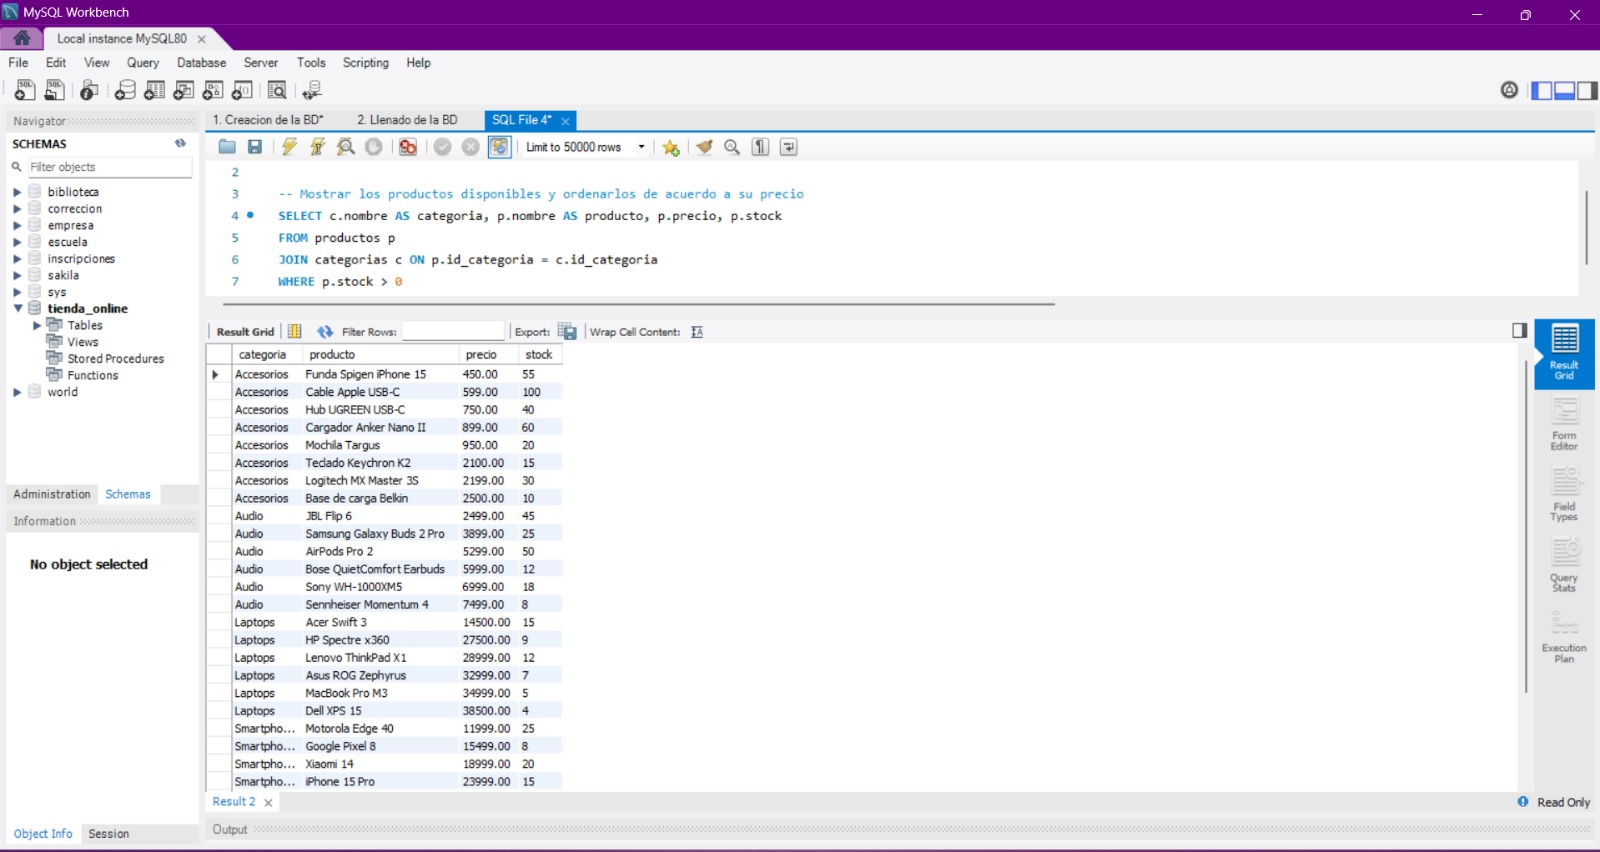
\includegraphics[width=\textwidth]{C1.1.jpeg}
    \end{subfigure}
    \hfill
    \begin{subfigure}{0.48\textwidth}
        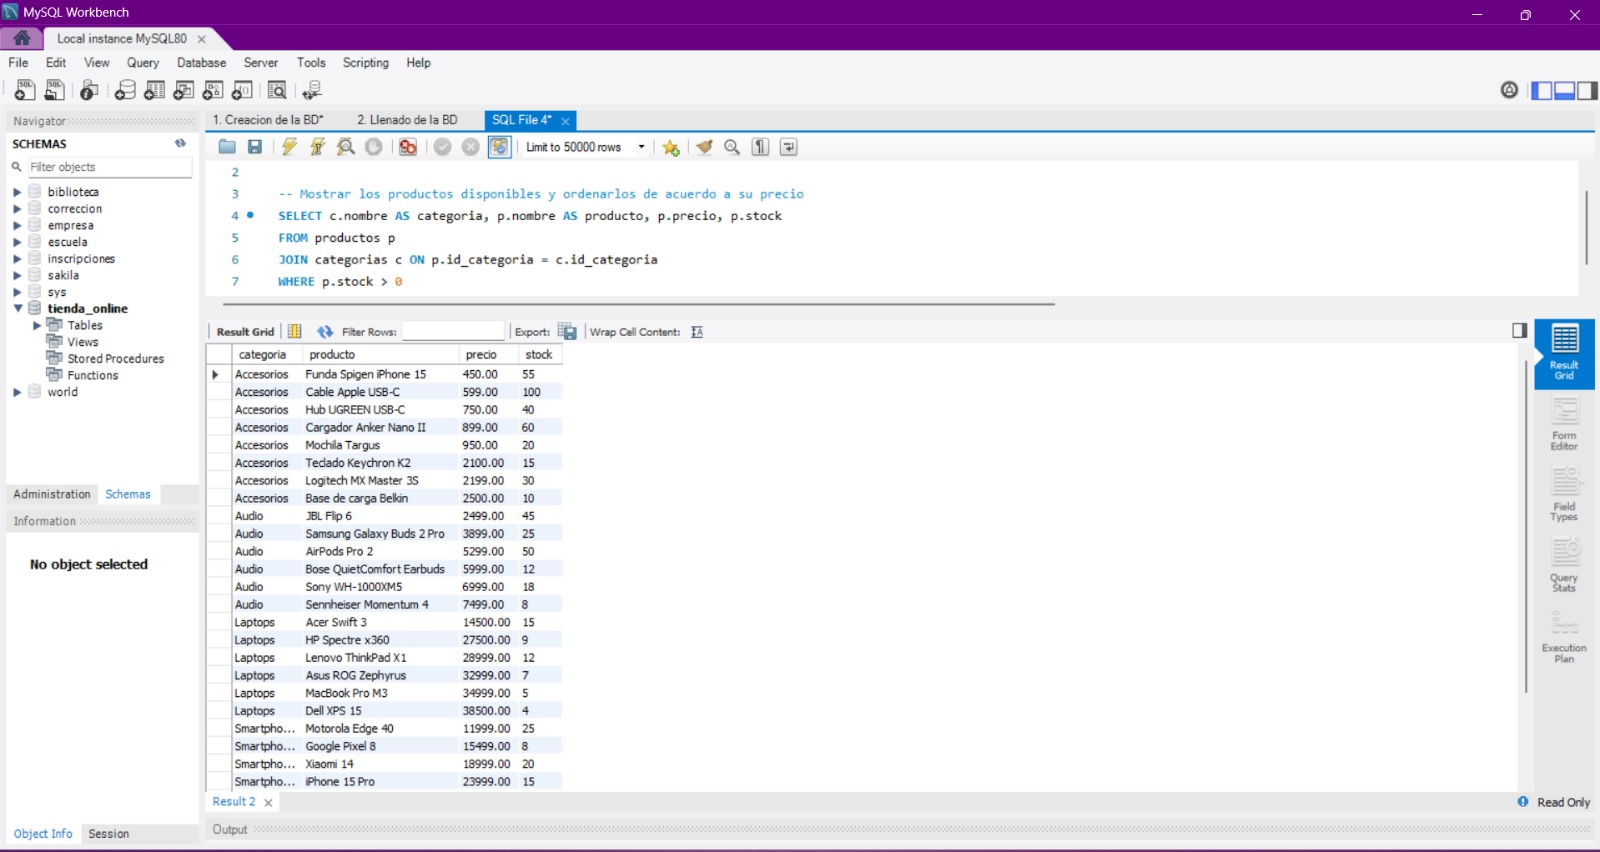
\includegraphics[width=\textwidth]{C1.1.jpeg}
    \end{subfigure}
    \caption{Resultados de la Consulta 1.}
\end{figure}

\subsection{Consulta 2: Clientes con pedidos pendientes y cuánto dinero gastaron}
\begin{lstlisting}
USE tienda_online;

-- Ver los clientes que mas dinero hann invertido y ver que pedidos tienen pendientes 
SELECT cl.nombre AS cliente, cl.correo,
       COUNT(DISTINCT pe.id_pedido) AS pedidos_pendientes,
       SUM(dp.cantidad * dp.precio_unitario) AS total_gastado
FROM clientes cl
JOIN pedidos pe ON cl.id_cliente = pe.id_cliente
JOIN detalles_pedido dp ON pe.id_pedido = dp.id_pedido
WHERE pe.estado = 'pendiente'
GROUP BY cl.id_cliente;
\end{lstlisting}
\begin{figure}[H]
    \centering
    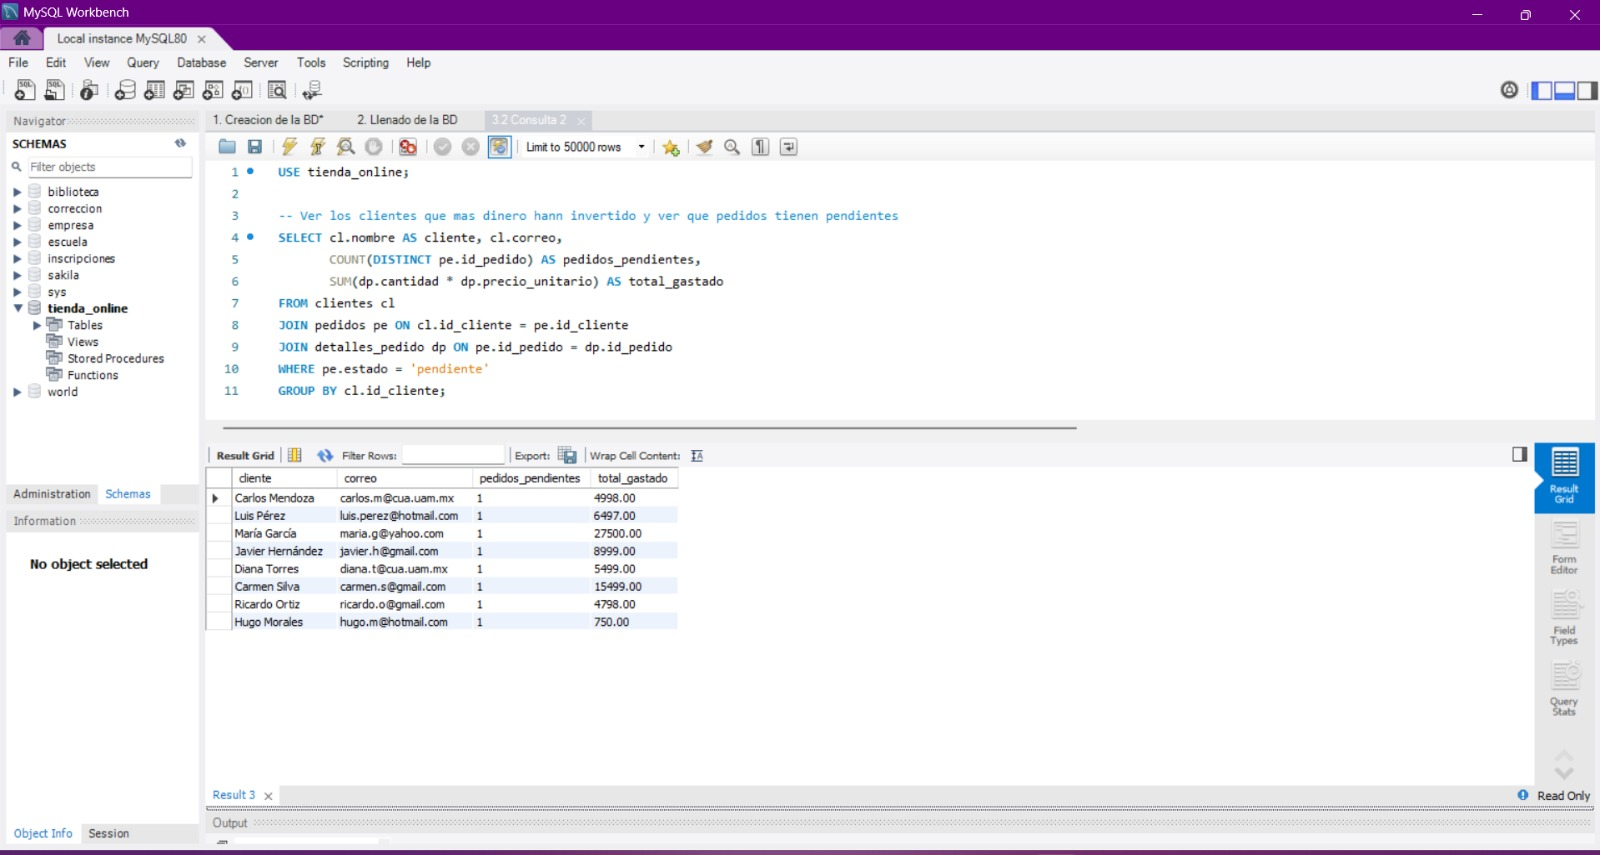
\includegraphics[width=0.9\textwidth]{C2.jpeg}
    \caption{Resultados de la Consulta 2.}
\end{figure}

\subsection{Consulta 3: Top 5 productos mejor calificados}
\begin{lstlisting}
USE tienda_online;

-- Mostrar los 5 productos mejor calificads 
SELECT p.nombre AS producto, ROUND(AVG(r.calificacion), 2) AS calificacion_promedio,
       COUNT(r.id_resena) AS total_resenas
FROM productos p
JOIN resenas r ON p.id_producto = r.id_producto
GROUP BY p.id_producto
ORDER BY calificacion_promedio DESC
LIMIT 5;
\end{lstlisting}
\begin{figure}[H]
    \centering
    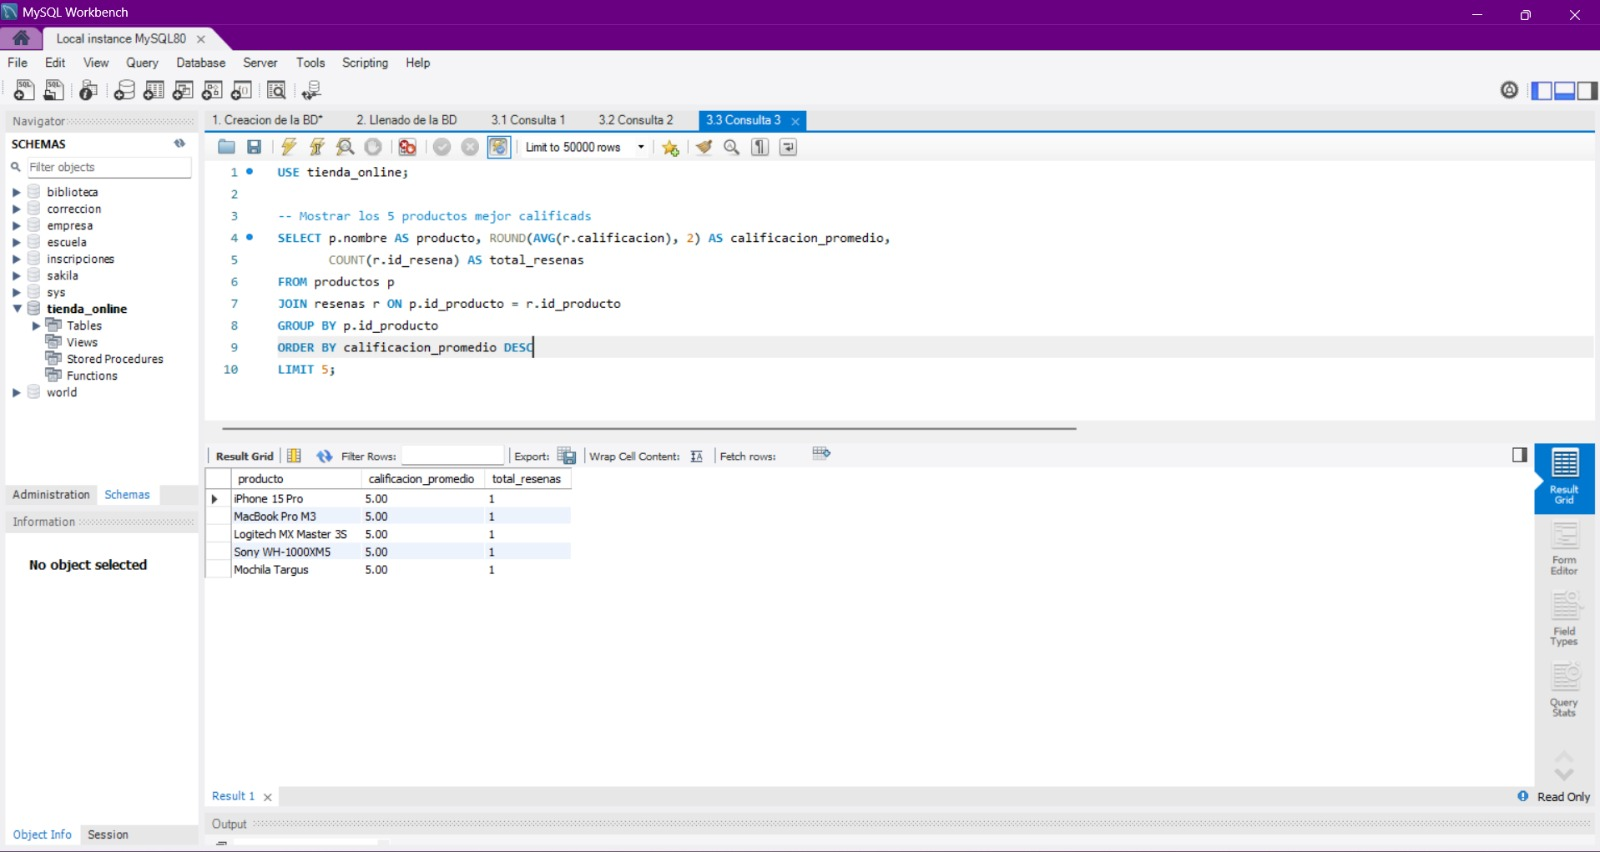
\includegraphics[width=0.9\textwidth]{C3.jpeg}
    \caption{Resultados de la Consulta 3.}
\end{figure}

\subsection{Consulta 4: Productos con necesidad de reabasteimiento}
\begin{lstlisting}
USE tienda_online;

-- Ver que productos es necesario reabastecer pronto
SELECT nombre, stock, id_categoria
FROM productos
WHERE stock < 5
ORDER BY stock ASC;
\end{lstlisting}
\begin{figure}[H]
    \centering
    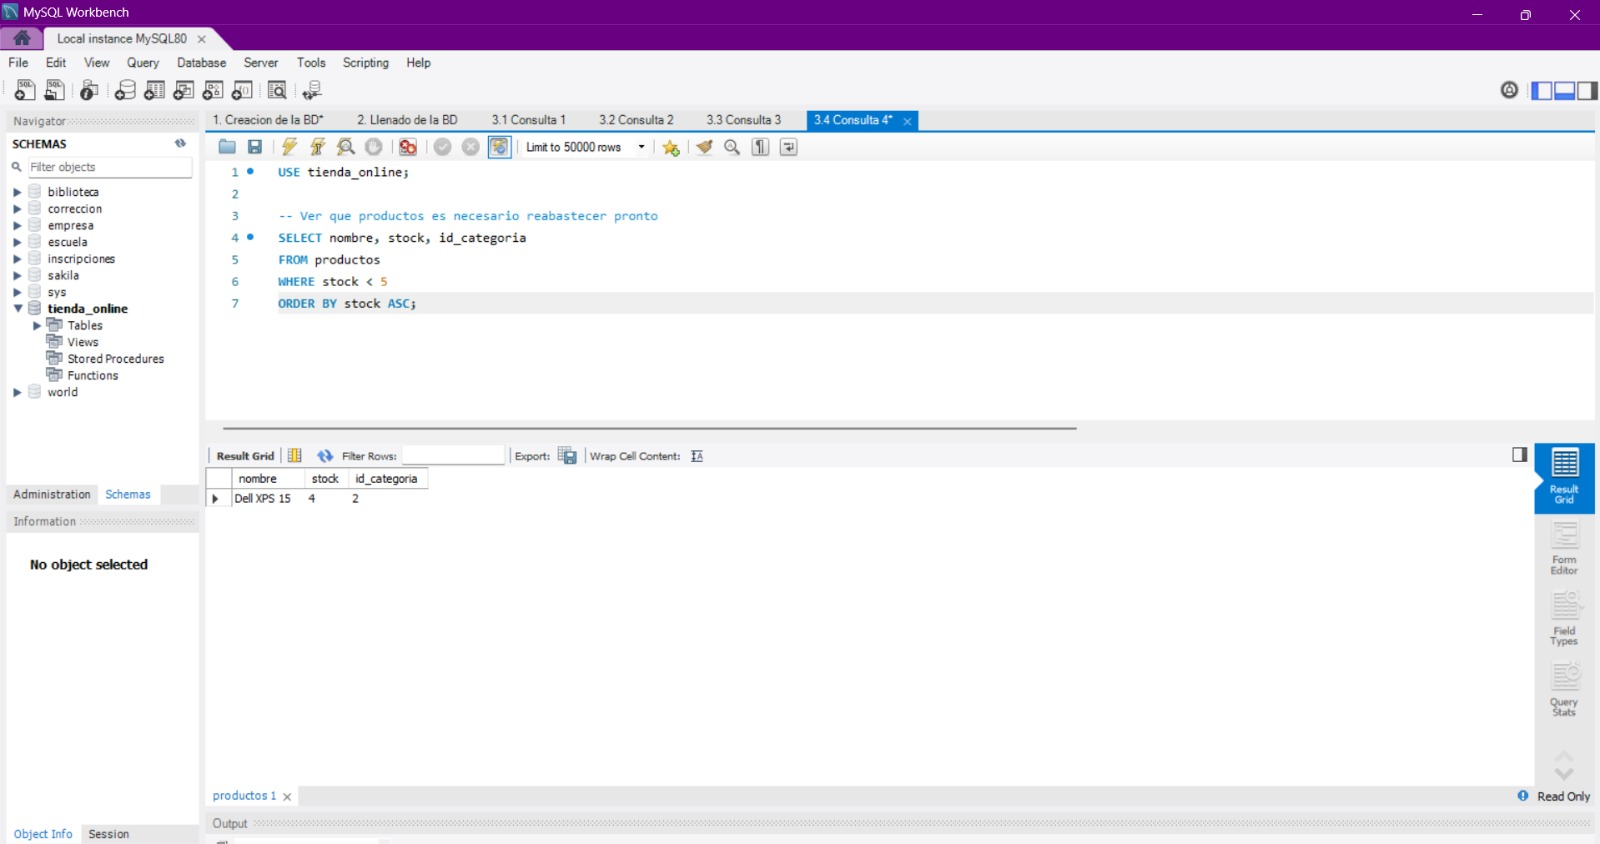
\includegraphics[width=0.9\textwidth]{C4.jpeg}
    \caption{Resultados de la Consulta 4.}
\end{figure}

\subsection{Consulta 5: Clientes recurrentes (con más de un pedido)}
\begin{lstlisting}
USE tienda_online;

-- Mostrar los clientes que han realizado mas de 1 pedido
SELECT cl.nombre, COUNT(pe.id_pedido) AS total_pedidos
FROM clientes cl
JOIN pedidos pe ON cl.id_cliente = pe.id_cliente
GROUP BY cl.id_cliente
HAVING total_pedidos > 1;
\end{lstlisting}
\begin{figure}[H]
    \centering
    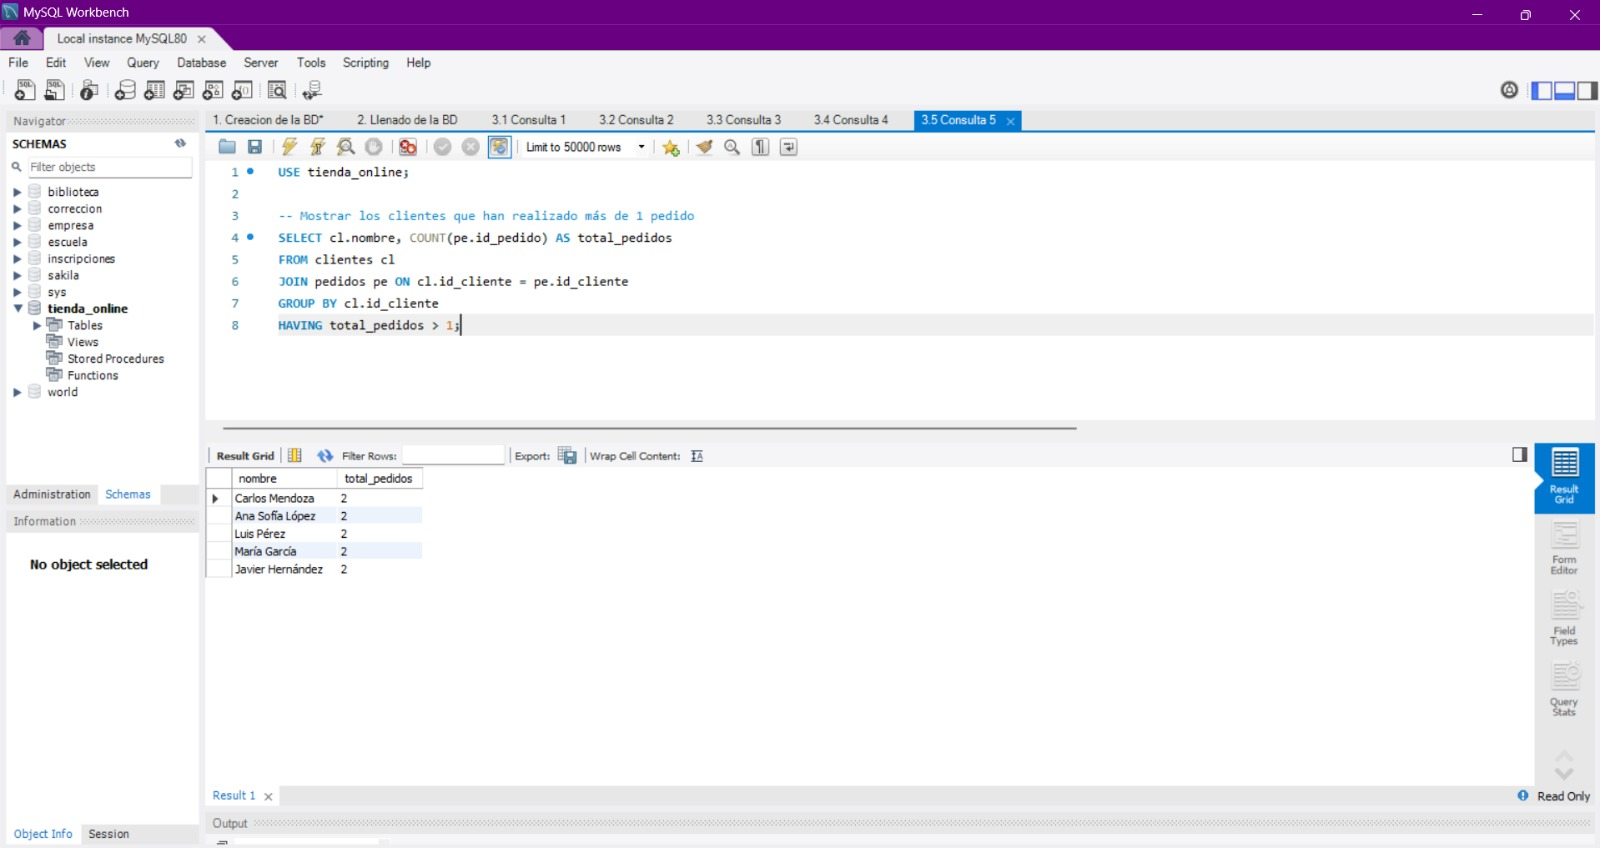
\includegraphics[width=0.9\textwidth]{C5.jpeg}
    \caption{Resultados de la Consulta 5.}
\end{figure}

\section{Procedimientos almacenados y validación}

\subsection{Procedimiento 1: Registrar nuevo pedido}
Valida el límite de compras y stock, posteriormente descuenta el inventario.
\begin{lstlisting}
USE tienda_online;
DROP PROCEDURE IF EXISTS RegistrarNuevoPedido;
DELIMITER //

CREATE PROCEDURE RegistrarNuevoPedido (
    IN p_cliente_id INT,
    IN p_producto_id INT,
    IN p_cantidad INT
)
BEGIN
    -- Declaramos variables para guardar lo que vamos a consultar
    DECLARE v_pendientes INT;
    DECLARE v_stock_actual INT;
    DECLARE v_precio DECIMAL(10,2);
    DECLARE v_nuevo_pedido_id INT;

    -- Primero verificamos la cantidad de pedidos pendientes que tiene el cliente
    SELECT COUNT(*) INTO v_pendientes
    FROM pedidos
    WHERE id_cliente = p_cliente_id AND estado = 'pendiente';

    -- Verificamos el stock y precio del producto slicitado 
    SELECT stock, precio INTO v_stock_actual, v_precio
    FROM productos
    WHERE id_producto = p_producto_id;

   -- Ponemos las condiciones para saber si se puede continuar o no con la compra
    IF v_pendientes >= 5 THEN
        -- Si tiene 5 pedidos pendientes, le mandamos un error
        SIGNAL SQLSTATE '45001' SET MESSAGE_TEXT = 'Error: Ya se tiene el maximo de pedidos pendientes';
        
    ELSEIF v_stock_actual < p_cantidad THEN
        -- Si pno tenemos stock suficiente, le mandamos un error
        SIGNAL SQLSTATE '45002' SET MESSAGE_TEXT = 'Error: Stock insuficiente para realizar el pedido.';
        
    ELSE
        -- Si se llego a este punto entonces realizamos el pedido 
        INSERT INTO pedidos (id_cliente, estado) VALUES (p_cliente_id, 'pendiente');
        
        -- Obtenemos el ID del pedido que se acaba de crear para poder usarlo como llave foranea 
        SET v_nuevo_pedido_id = LAST_INSERT_ID();

        -- Insertamos la nueva informacion en la tabla de detalles_pedido
        INSERT INTO detalles_pedido (id_pedido, id_producto, cantidad, precio_unitario)
        VALUES (v_nuevo_pedido_id, p_producto_id, p_cantidad, v_precio);

        -- Decrementamos el stock para futuras compras 
        UPDATE productos
        SET stock = stock - p_cantidad
        WHERE id_producto = p_producto_id;
        
    END IF;
END //

DELIMITER ;
\end{lstlisting}
\begin{figure}[H]
    \centering
    \begin{subfigure}{0.32\textwidth}
        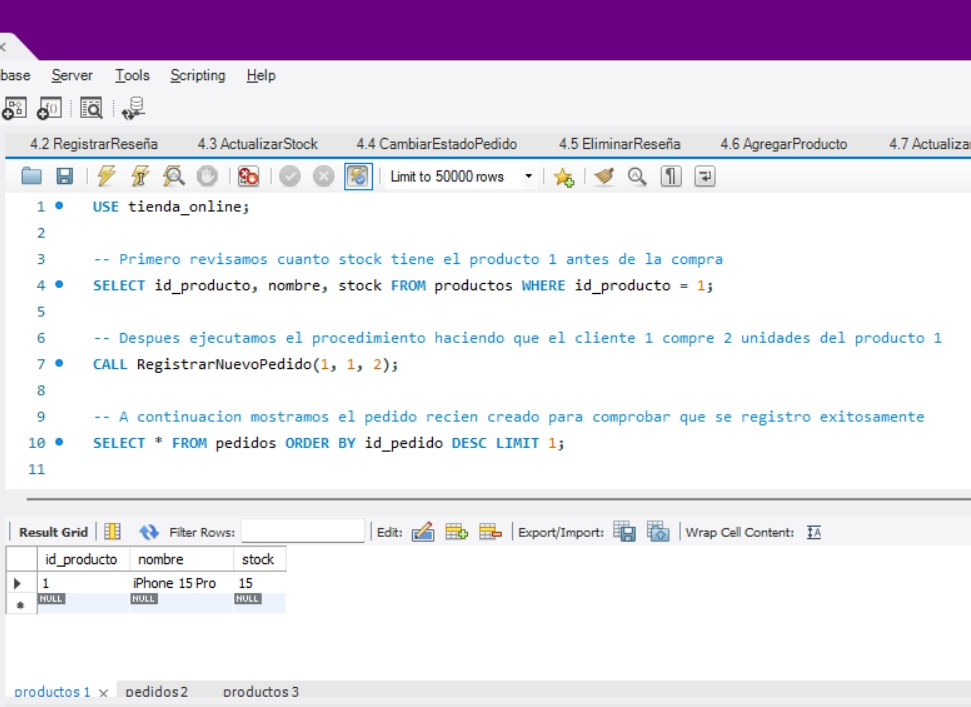
\includegraphics[width=\textwidth]{PRU1.1.jpeg}
        \caption{Stock antes}
    \end{subfigure}
    \hfill
    \begin{subfigure}{0.32\textwidth}
        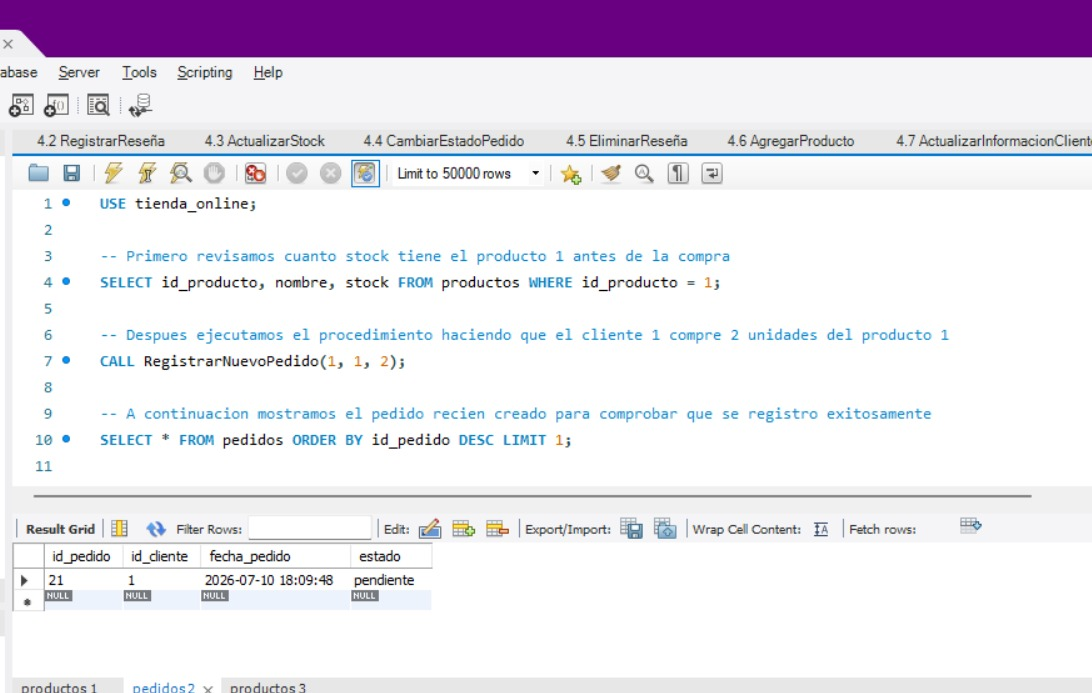
\includegraphics[width=\textwidth]{PRU1.2.jpeg}
        \caption{Ejecución}
    \end{subfigure}
    \hfill
    \begin{subfigure}{0.32\textwidth}
        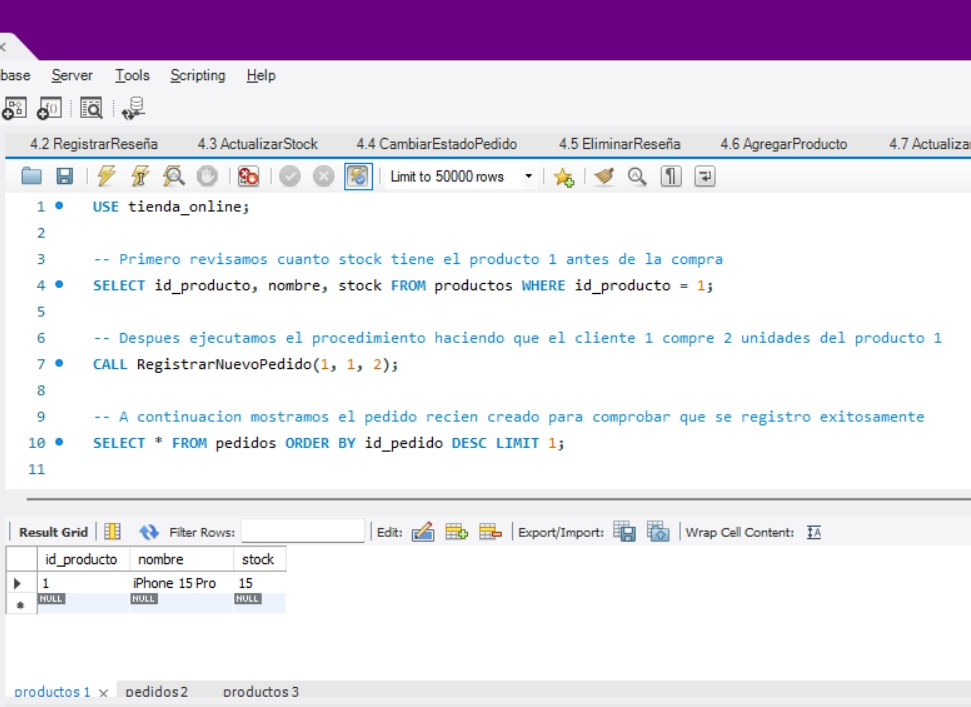
\includegraphics[width=\textwidth]{PRU1.1.jpeg}
        \caption{Stock después}
    \end{subfigure}
    \caption{Flujo del Procedimiento 1.}
\end{figure}

\subsection{Procedimiento 2: Registrar reseña}
Comprueba que el cliente haya comprado el artículo. Si no, arroja error.
\begin{lstlisting}
USE tienda_online;
DROP PROCEDURE IF EXISTS RegistrarResena;
DELIMITER //

CREATE PROCEDURE RegistrarResena (
    IN p_cliente_id INT,
    IN p_producto_id INT,
    IN p_calificacion INT,
    IN p_comentario TEXT
)
BEGIN
    -- Declaramos una variable para guardar la cantidad de veces que ha comprado el producto
    DECLARE v_comprado INT;

    -- Primero buscamos en los pedidos para confirmar que el cliente realmente compro este producto
    SELECT COUNT(*) INTO v_comprado
    FROM pedidos p
    JOIN detalles_pedido dp ON p.id_pedido = dp.id_pedido
    WHERE p.id_cliente = p_cliente_id AND dp.id_producto = p_producto_id;

    -- Ponemos las condiciones para saber si se puede continuar
    IF v_comprado = 0 THEN
        -- Si no lo ha comprado, le mandamos un error
        SIGNAL SQLSTATE '45003' SET MESSAGE_TEXT = 'Error: No se puede dar resena de un producto no comprado';
        
    ELSE
        -- Si se llego a este punto entonces guardamos la resena en la tabla
        INSERT INTO resenas (id_cliente, id_producto, calificacion, comentario)
        VALUES (p_cliente_id, p_producto_id, p_calificacion, p_comentario);
        
    END IF;
END //

DELIMITER ;
\end{lstlisting}
\begin{figure}[H]
    \centering
    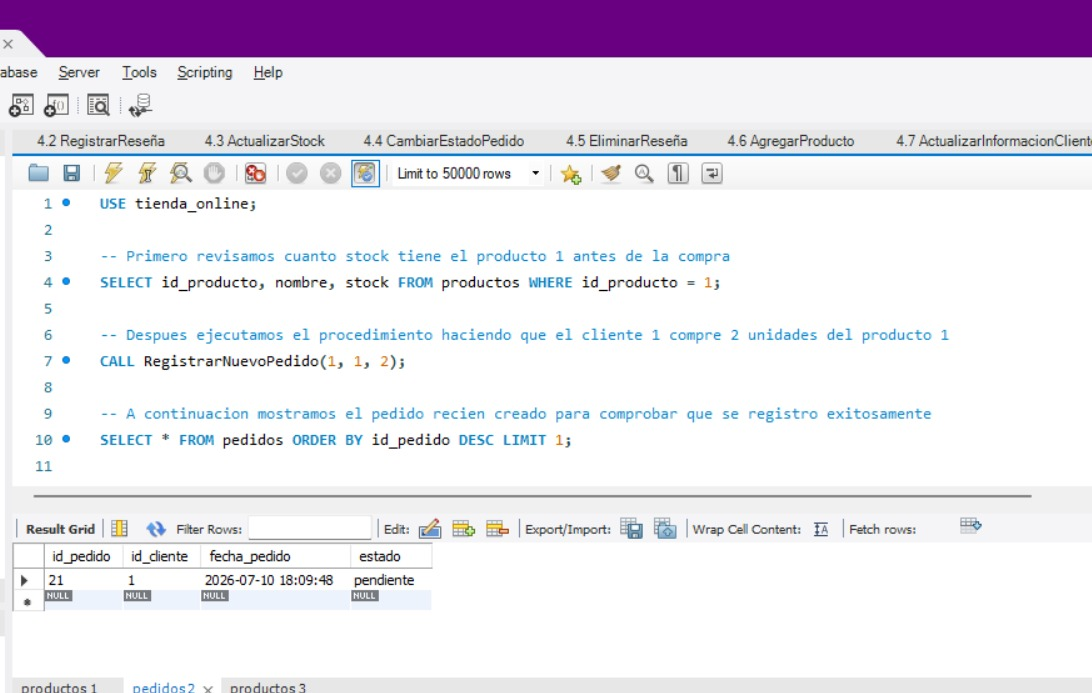
\includegraphics[width=0.9\textwidth]{PRU1.2.jpeg}
    \caption{Bloqueo del sistema al intentar reseñar sin compra.}
\end{figure}

\subsection{Procedimiento 3: Actualizar stock}
\begin{lstlisting}
USE tienda_online;
DROP PROCEDURE IF EXISTS ActualizarStock;
DELIMITER //

CREATE PROCEDURE ActualizarStock (
    IN p_producto_id INT,
    IN p_cantidad INT
)
BEGIN
    -- Descontamos la cantidad solicitada del inventario actual del producto
    UPDATE productos
    SET stock = stock - p_cantidad
    WHERE id_producto = p_producto_id;
END //

DELIMITER ;
\end{lstlisting}
\begin{figure}[H]
    \centering
    \begin{subfigure}{0.48\textwidth}
        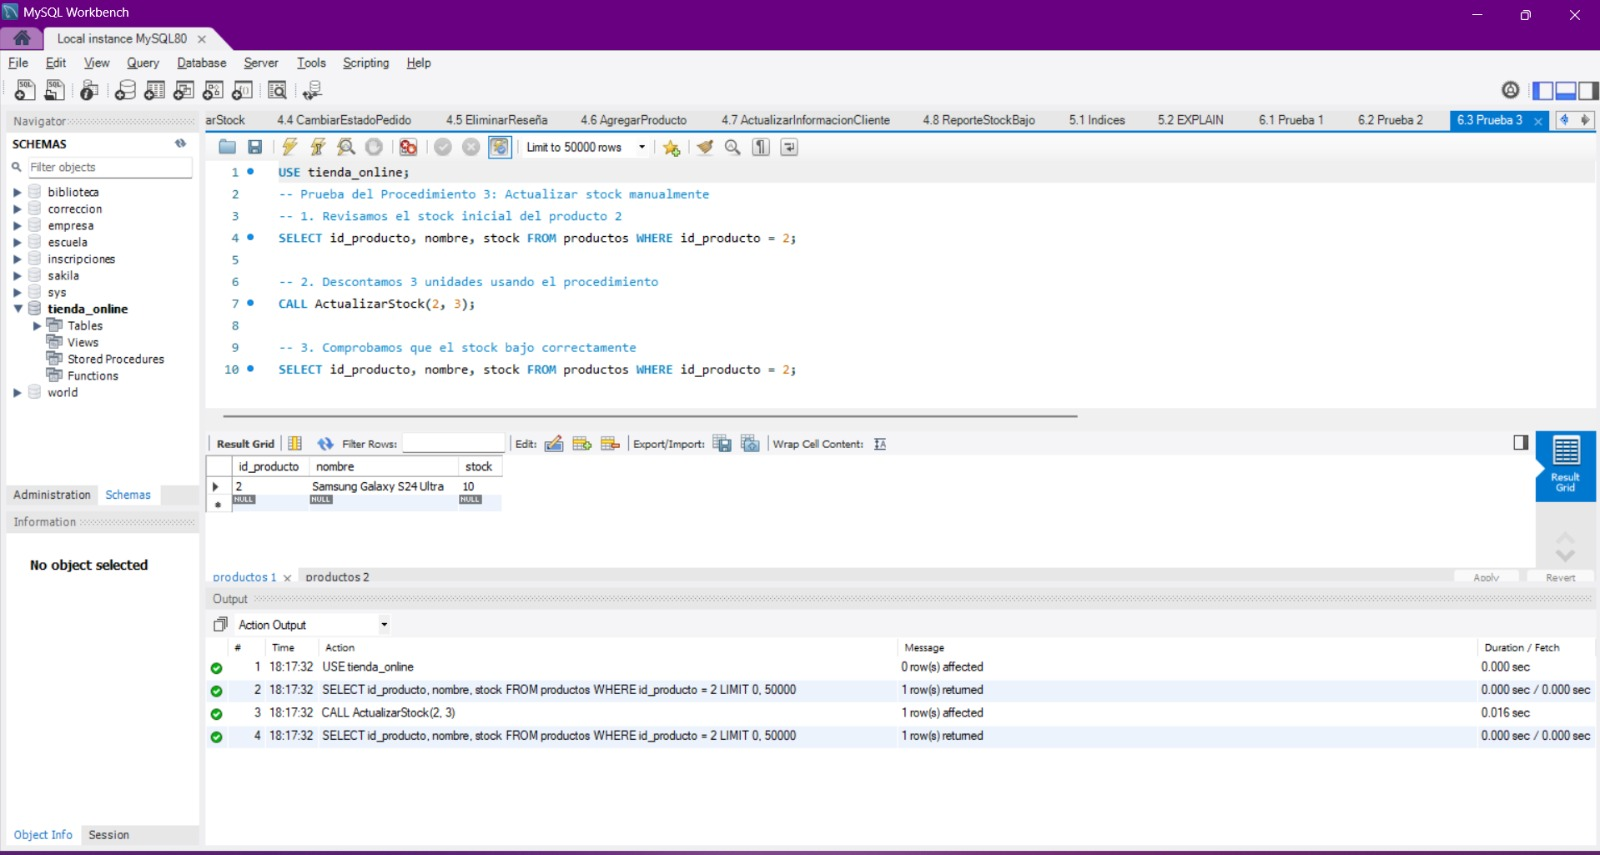
\includegraphics[width=\textwidth]{PRU3.1.jpeg}
        \caption{Stock antes de ajuste}
    \end{subfigure}
    \hfill
    \begin{subfigure}{0.48\textwidth}
        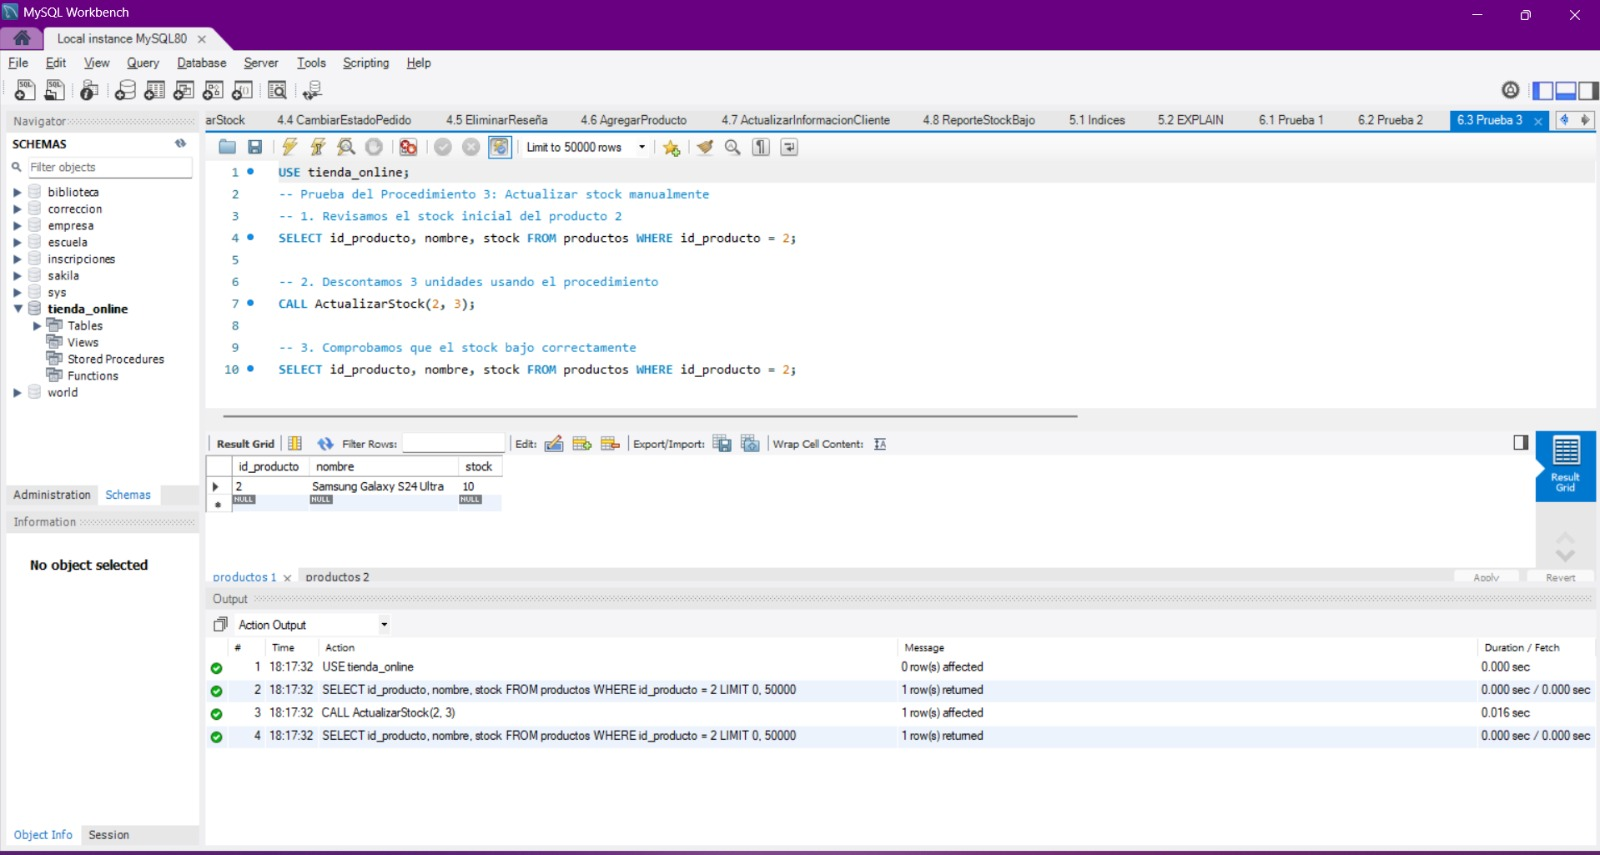
\includegraphics[width=\textwidth]{PRU3.1.jpeg}
        \caption{Stock actualizado}
    \end{subfigure}
\end{figure}

\subsection{Procedimiento 4: Cambiar estado de pedido}
\begin{lstlisting}
USE tienda_online;

DROP PROCEDURE IF EXISTS CambiarEstadoPedido;
DELIMITER //

CREATE PROCEDURE CambiarEstadoPedido (
    IN p_pedido_id INT,
    IN p_nuevo_estado VARCHAR(20)
)
BEGIN
    -- Actualizamos el estado del pedido al nuevo valor solicitado
    UPDATE pedidos
    SET estado = p_nuevo_estado
    WHERE id_pedido = p_pedido_id;
END //

DELIMITER ;
\end{lstlisting}
\begin{figure}[H]
    \centering
    \begin{subfigure}{0.48\textwidth}
        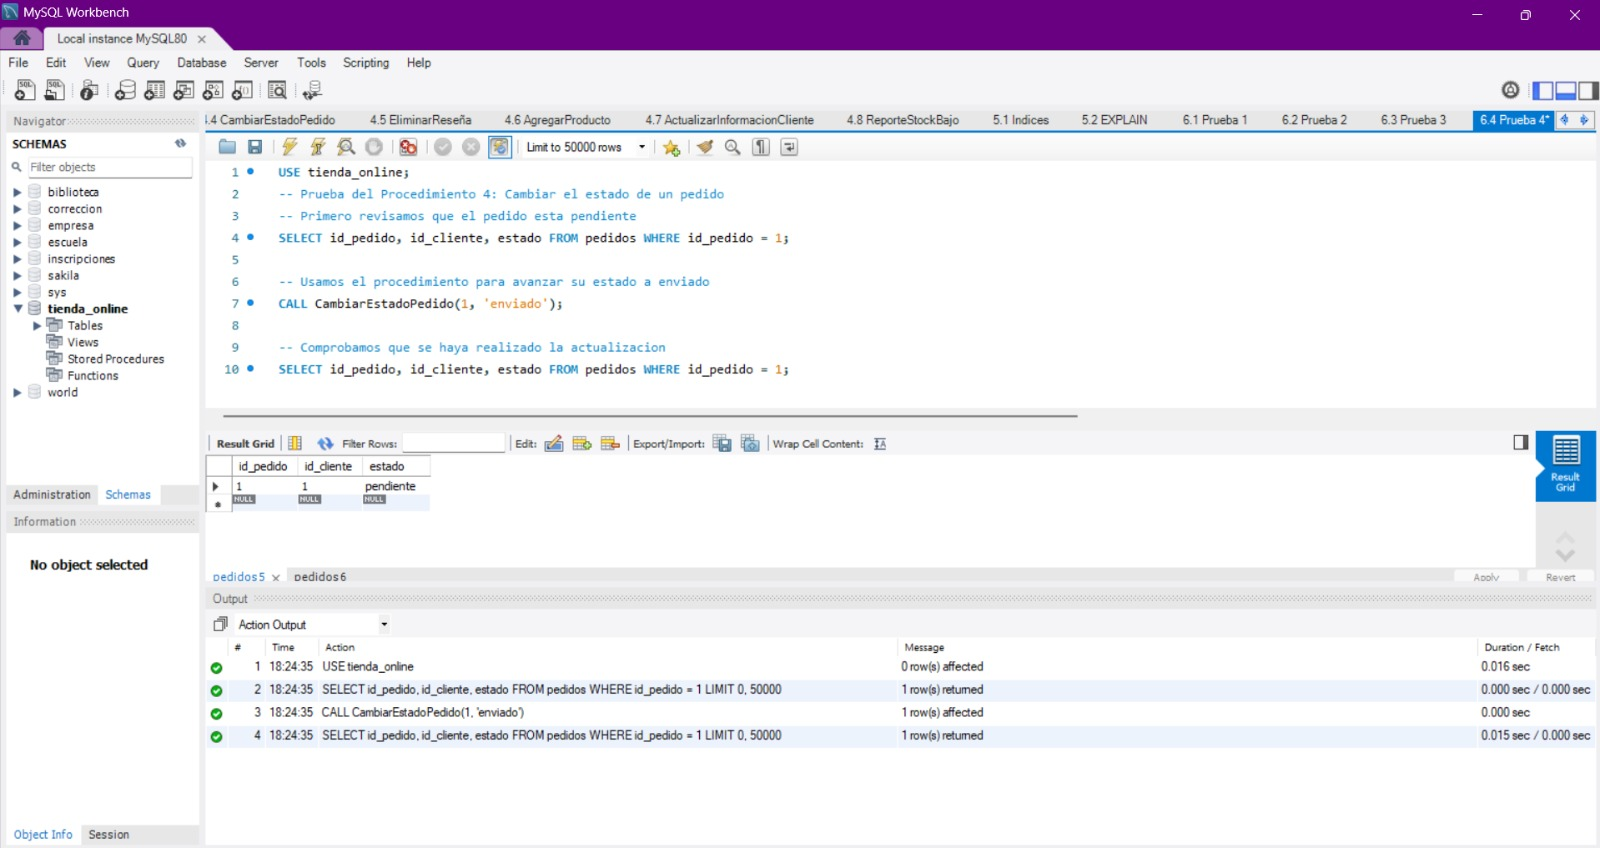
\includegraphics[width=\textwidth]{PRU4.1.jpeg}
        \caption{Estado Pendiente}
    \end{subfigure}
    \hfill
    \begin{subfigure}{0.48\textwidth}
        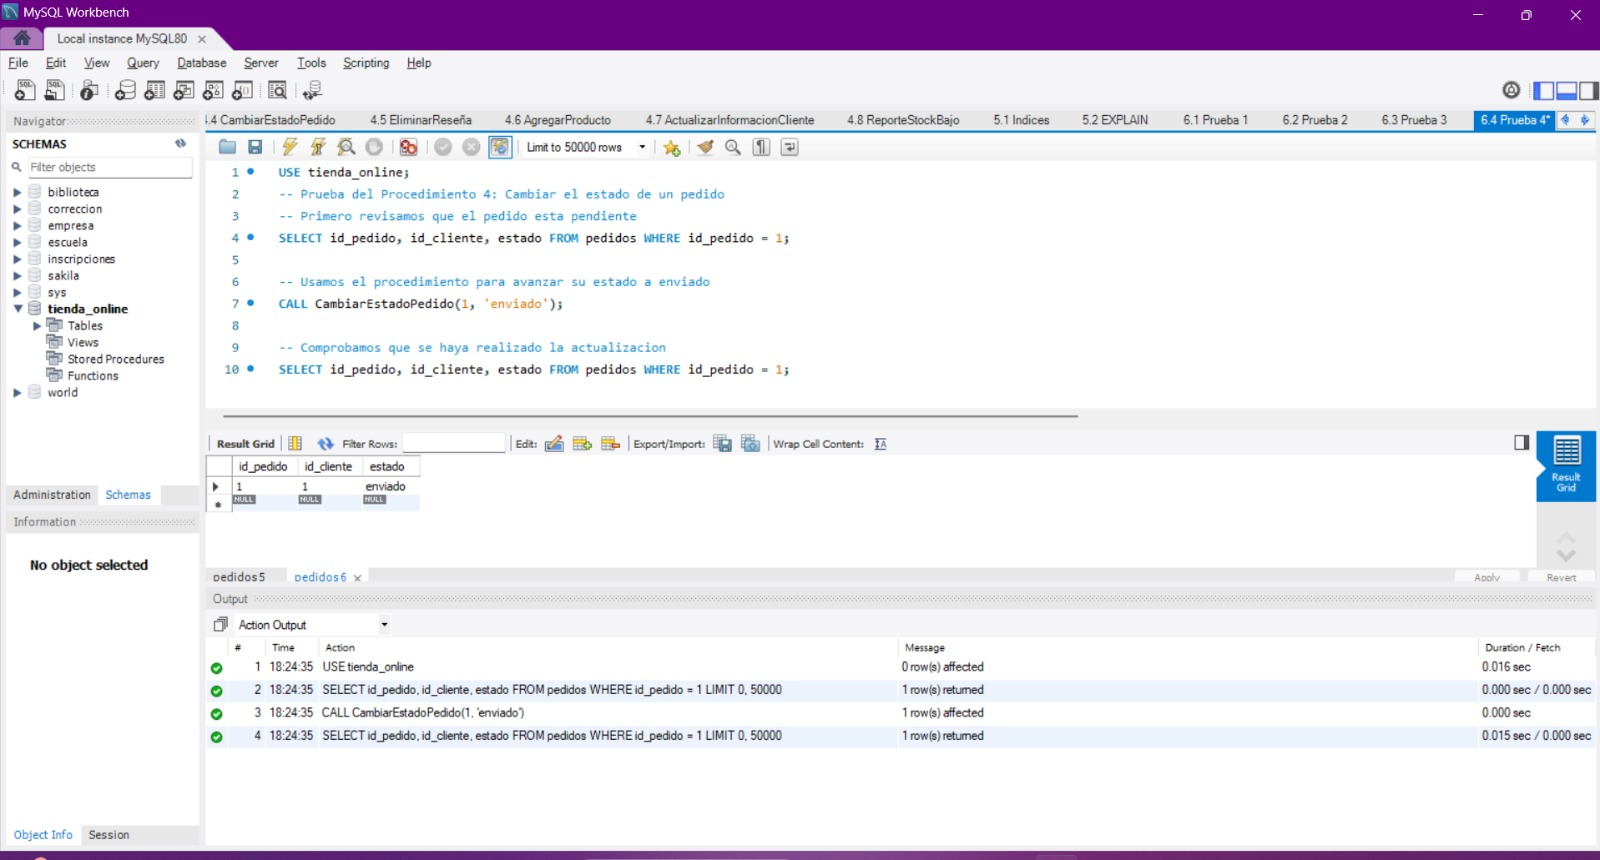
\includegraphics[width=\textwidth]{PRU4.2.jpeg}
        \caption{Estado Enviado}
    \end{subfigure}
\end{figure}

\subsection{Procedimiento 5: Eliminar eeseña}
Borra la calificación y recalcula el promedio general del producto.
\begin{lstlisting}
Use tienda_online;
DROP PROCEDURE IF EXISTS EliminarResena;
DELIMITER //

CREATE PROCEDURE EliminarResena (
    IN p_resena_id INT
)
BEGIN
    -- Declaramos una variable para guardar el producto al que pertenece la resena
    DECLARE v_producto_id INT;

    -- Primero obtenemos el id del producto antes de borrar la resena para no perder el dato
    SELECT id_producto INTO v_producto_id
    FROM resenas
    WHERE id_resena = p_resena_id;

    -- Despues eliminamos la resena de la tabla
    DELETE FROM resenas
    WHERE id_resena = p_resena_id;

    -- A continuacion calculamos y mostramos el nuevo promedio de ese producto actualizado
    SELECT id_producto, AVG(calificacion) AS nuevo_promedio
    FROM resenas
    WHERE id_producto = v_producto_id
    GROUP BY id_producto;
END //

DELIMITER ;
\end{lstlisting}
\begin{figure}[H]
    \centering
    \begin{subfigure}{0.32\textwidth}
        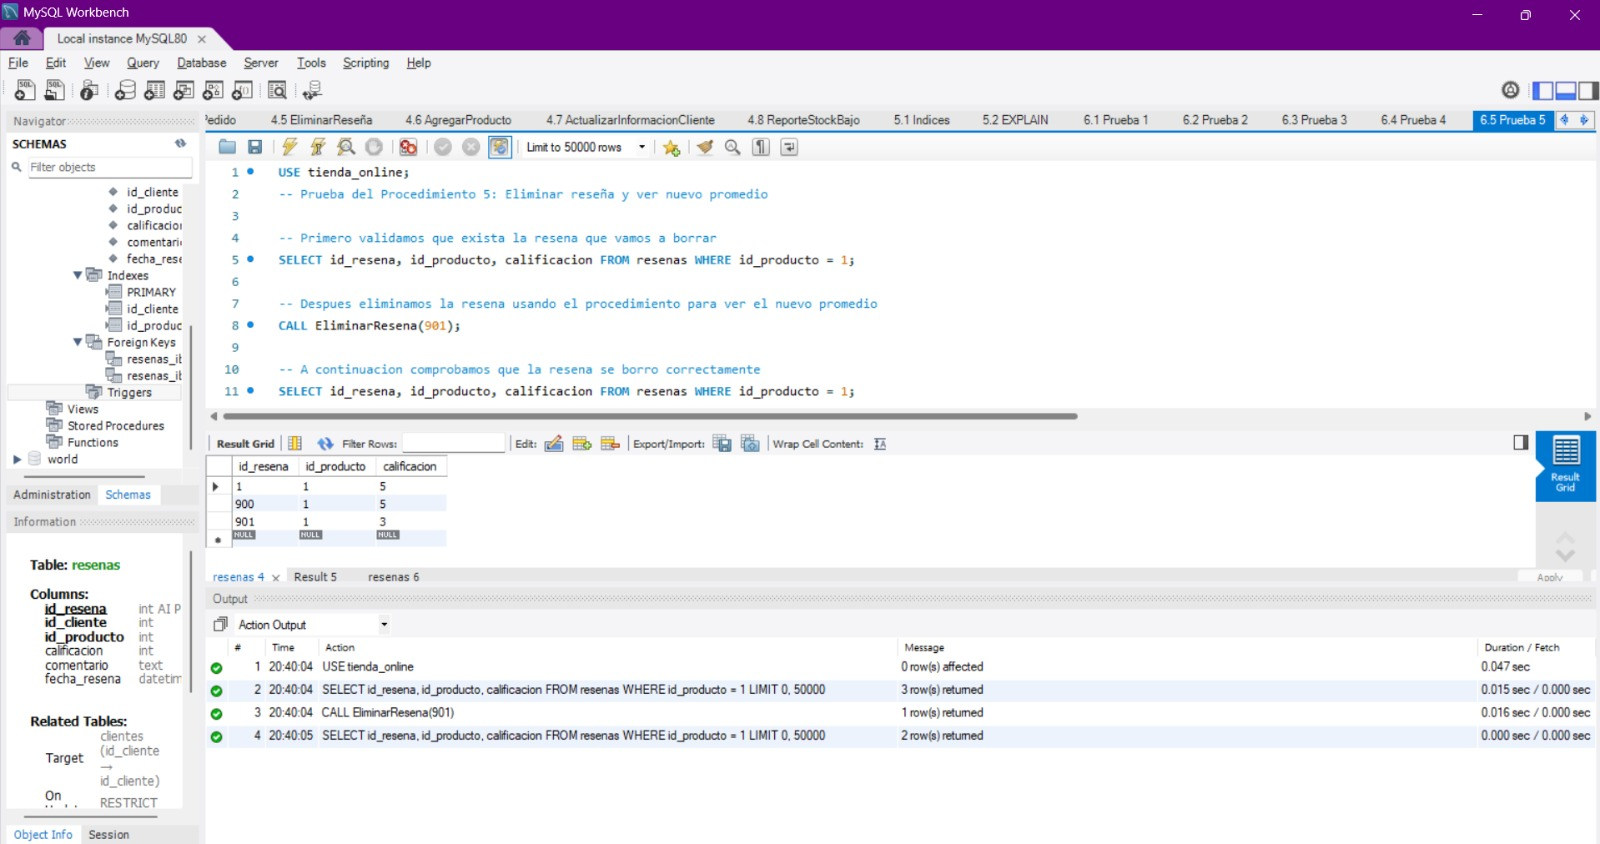
\includegraphics[width=\textwidth]{PRU5.1.jpeg}
    \end{subfigure}
    \hfill
    \begin{subfigure}{0.32\textwidth}
        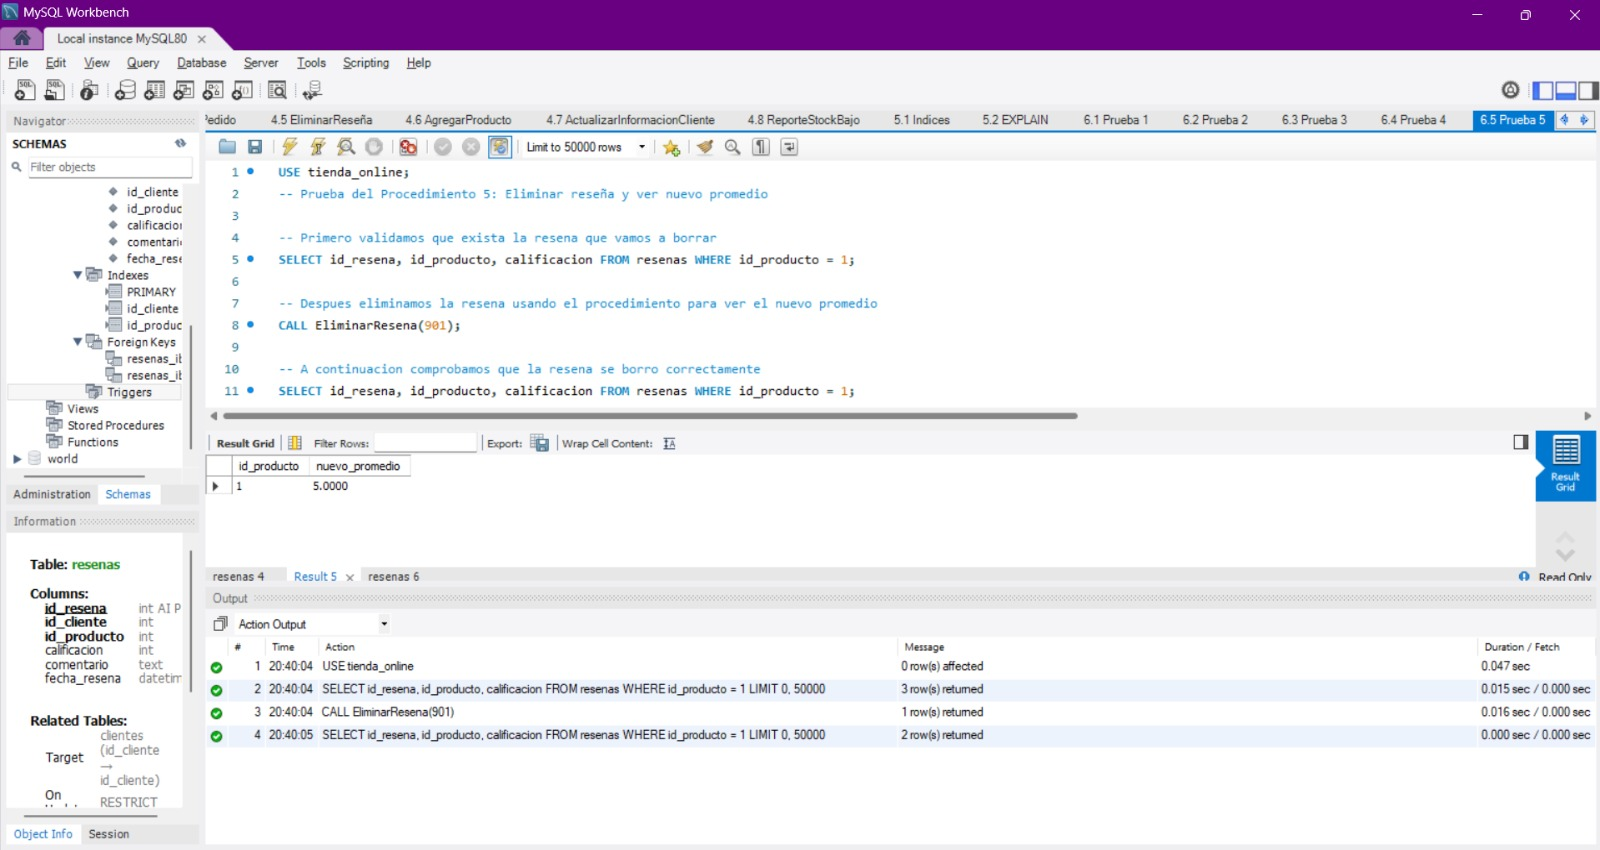
\includegraphics[width=\textwidth]{PRU5.2.jpeg}
    \end{subfigure}
    \hfill
    \begin{subfigure}{0.32\textwidth}
        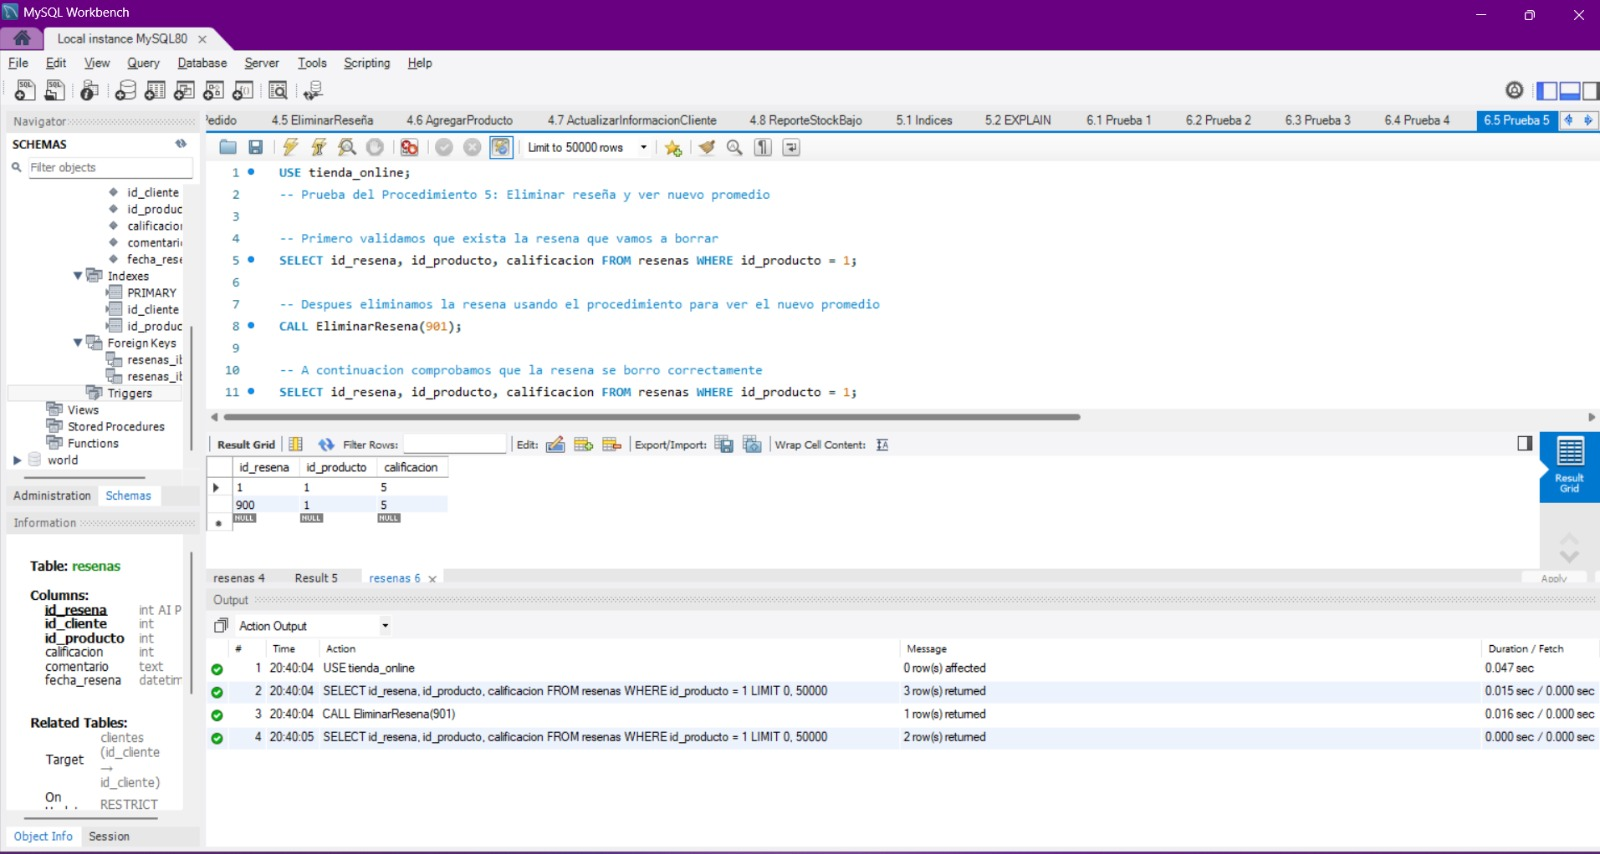
\includegraphics[width=\textwidth]{PRU5.3.jpeg}
    \end{subfigure}
    \caption{Proceso de eliminación y recálculo de promedio.}
\end{figure}

\subsection{Procedimiento 6: Agregar producto (validar duplicados)}
\begin{lstlisting}
USE tienda_online;
DROP PROCEDURE IF EXISTS AgregarProducto;
DELIMITER //

CREATE PROCEDURE AgregarProducto (
    IN p_nombre VARCHAR(50),
    IN p_descripcion TEXT,
    IN p_precio DECIMAL(10,2),
    IN p_stock INT,
    IN p_categoria_id INT
)
BEGIN
    -- Declaramos una variable para comprobar si el producto ya esta registrado
    DECLARE v_existe INT;

    -- Primero contamos si hay algun producto que tenga exactamente el mismo nombre y categoria
    SELECT COUNT(*) INTO v_existe
    FROM productos
    WHERE nombre = p_nombre AND id_categoria = p_categoria_id;

    -- Ponemos la condicion para evitar duplicados
    IF v_existe > 0 THEN
        -- Si el contador detecta que ya existe, mandamos un error
        SIGNAL SQLSTATE '45004' SET MESSAGE_TEXT = 'Error: El producto ya existe en esta categoria';
        
    ELSE
        -- Si no existe, entonces lo insertamos normalmente en el inventario
        INSERT INTO productos (nombre, descripcion, precio, stock, id_categoria)
        VALUES (p_nombre, p_descripcion, p_precio, p_stock, p_categoria_id);
        
    END IF;
END //

DELIMITER ;
\end{lstlisting}
\begin{figure}[H]
    \centering
    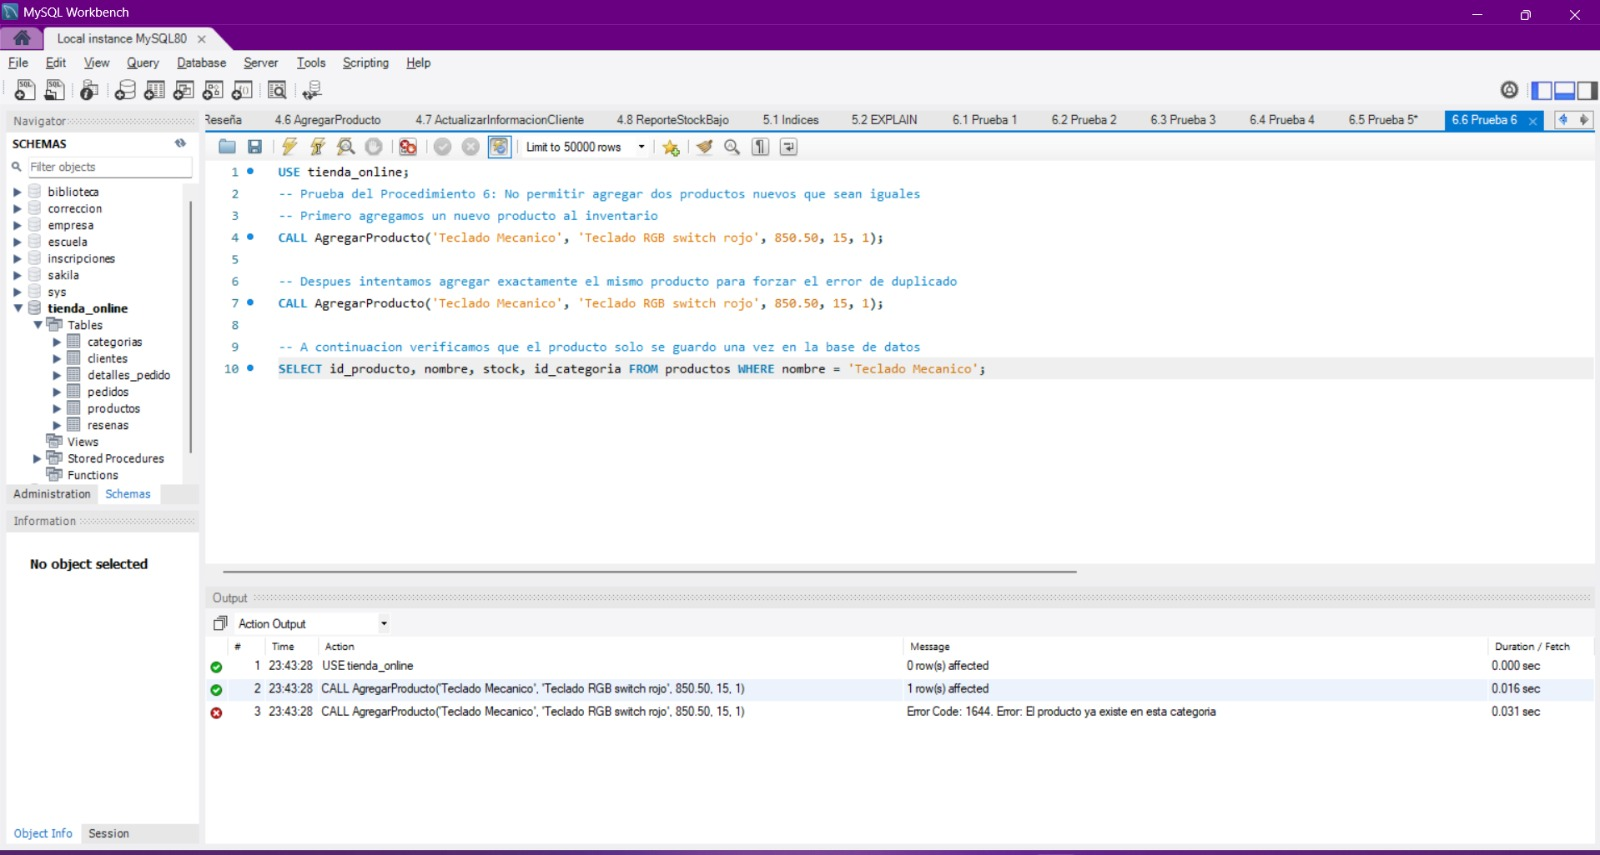
\includegraphics[width=0.9\textwidth]{PRU6.jpeg}
    \caption{Validación correcta y no aceptacion del producto "duplicado"}
\end{figure}

\subsection{Procedimiento 7: Actualizar Información de Cliente}
\begin{lstlisting}
USE tienda_online;
DROP PROCEDURE IF EXISTS ActualizarCliente;
DELIMITER //

CREATE PROCEDURE ActualizarCliente (
    IN p_cliente_id INT,
    IN p_telefono VARCHAR(10),
    IN p_direccion TEXT
)
BEGIN
    -- Actualizamos la informacion de contacto del cliente en la base de datos
    UPDATE clientes
    SET telefono = p_telefono, 
        direccion = p_direccion
    WHERE id_cliente = p_cliente_id;
END //

DELIMITER ;
\end{lstlisting}
\begin{figure}[H]
    \centering
    \begin{subfigure}{0.48\textwidth}
        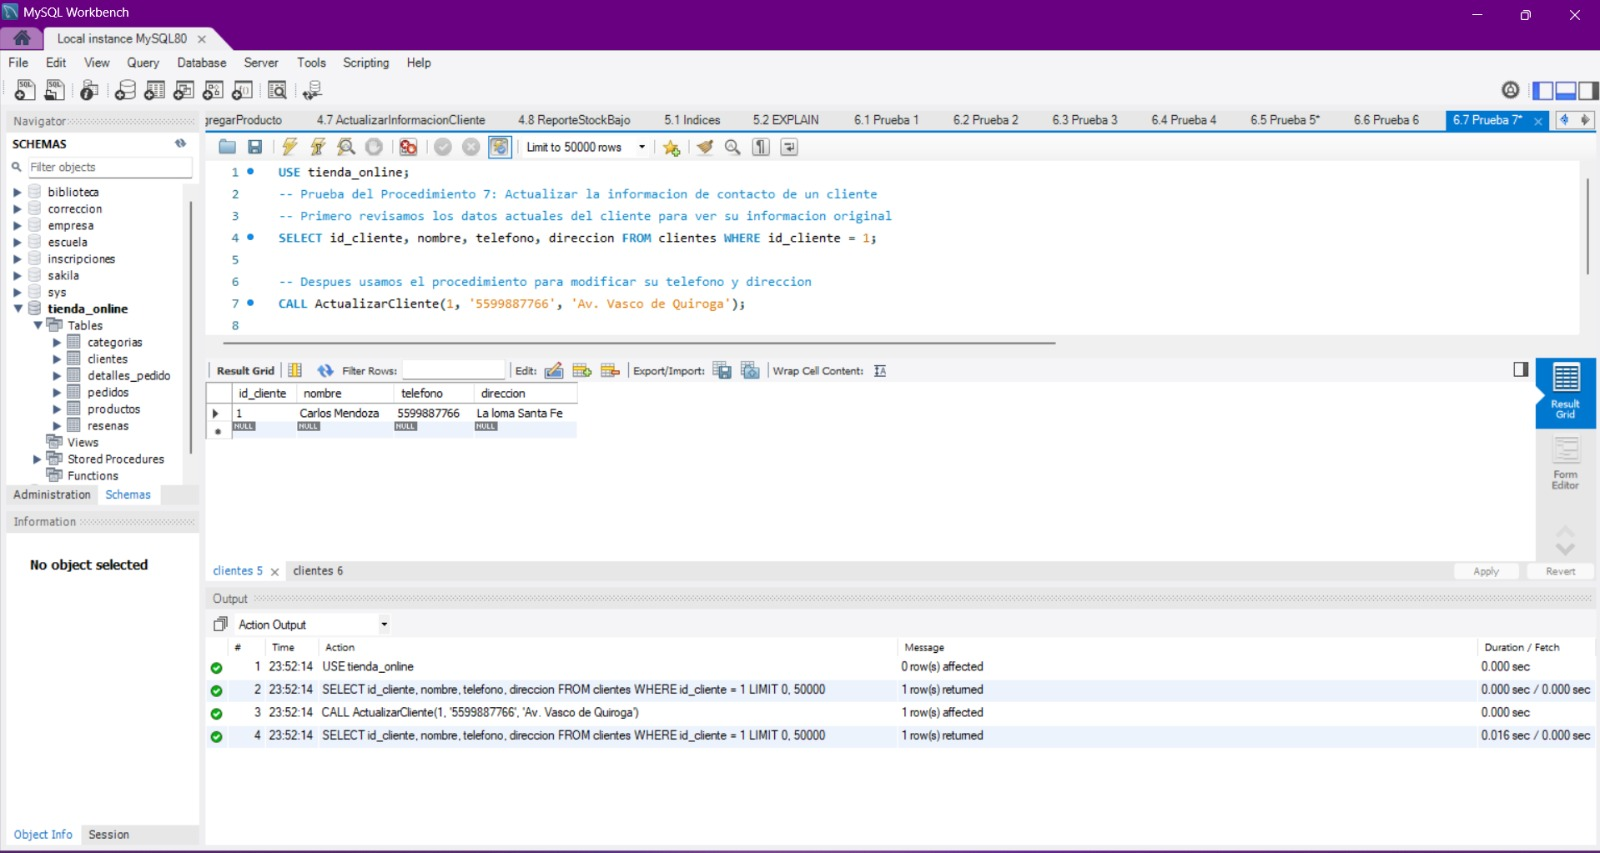
\includegraphics[width=\textwidth]{PRU7.1.jpeg}
    \end{subfigure}
    \hfill
    \begin{subfigure}{0.48\textwidth}
        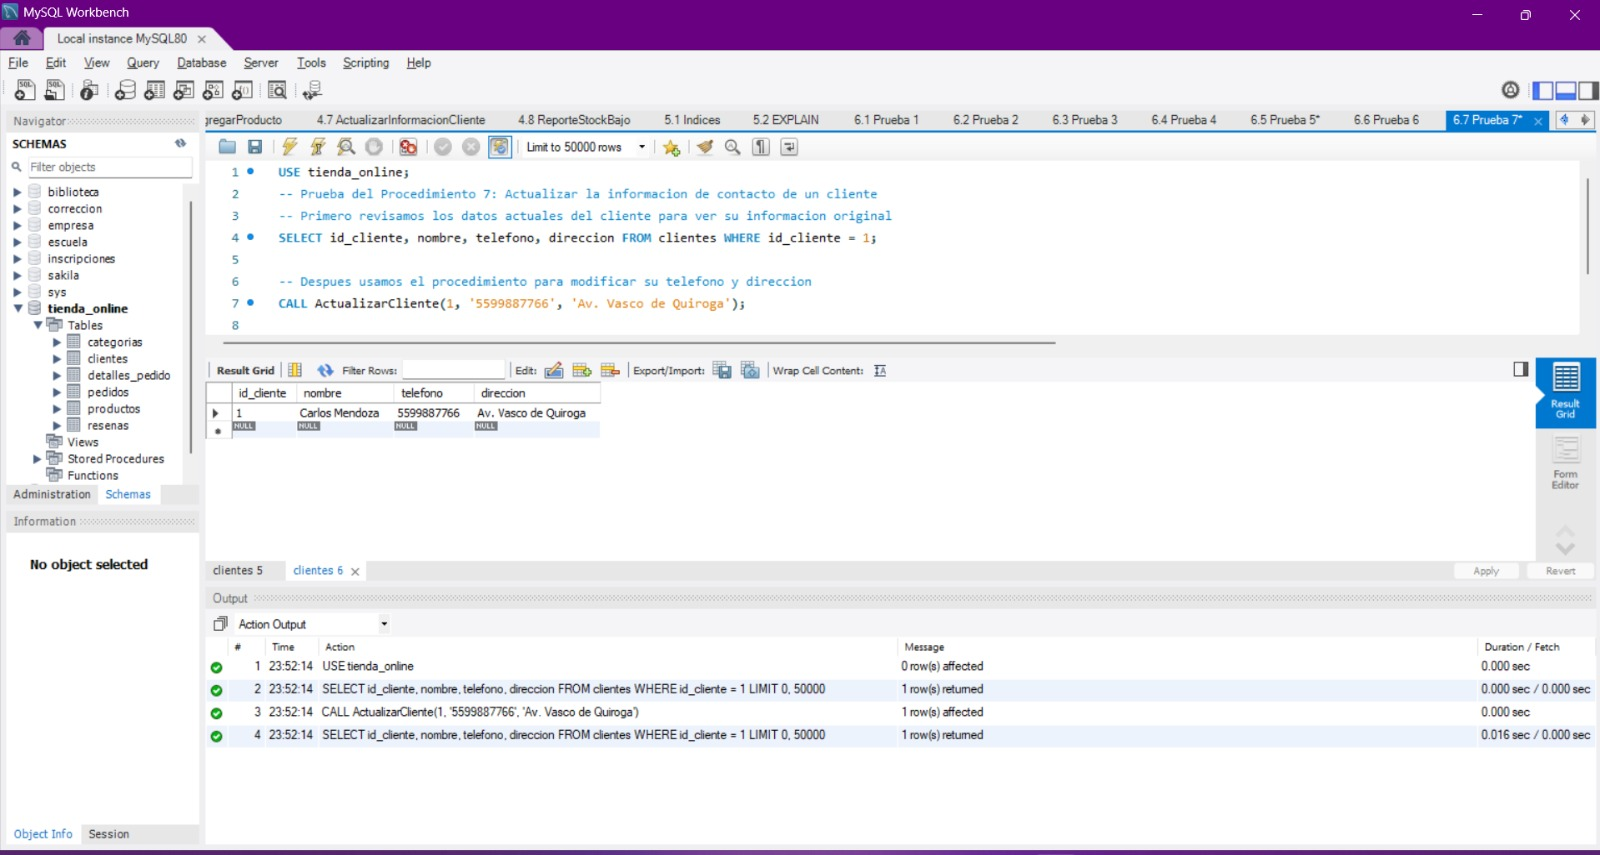
\includegraphics[width=\textwidth]{PRU7.2.jpeg}
    \end{subfigure}
    \caption{Actualización de datos del cliente.}
\end{figure}

\subsection{Procedimiento 8: Reporte de Stock Bajo}
\begin{lstlisting}
USE tienda_online;
DROP PROCEDURE IF EXISTS ReporteStockBajo;
DELIMITER //

CREATE PROCEDURE ReporteStockBajo ()
BEGIN
    -- Generamos un reporte mostrando los productos que tienen menos de 5 unidades en inventario
    SELECT id_producto, nombre, stock, id_categoria
    FROM productos
    WHERE stock < 5
    ORDER BY stock ASC;
END //

DELIMITER ;
\end{lstlisting}
\begin{figure}[H]
    \centering
    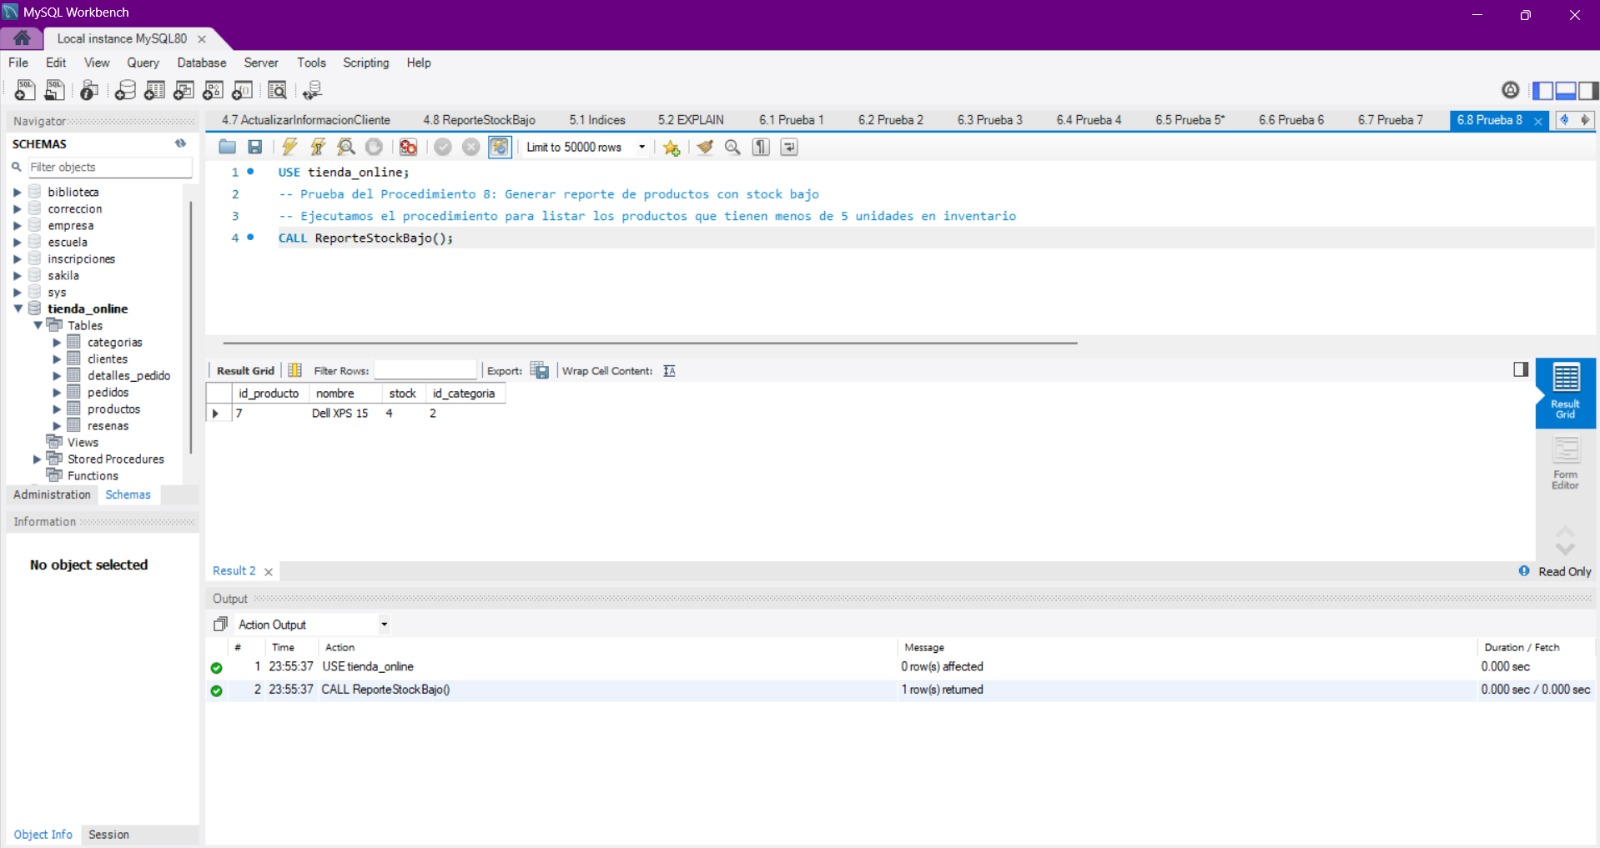
\includegraphics[width=0.9\textwidth]{PRU8.jpeg}
    \caption{Lista de productos con stock bajo}
\end{figure}


\section{Optimización y rendimiento}

\subsection{Creación de indices}
Para asegurar la escalabilidad del sistema, se crearon indices para las consultas más frecuentes.
\begin{lstlisting}
USE tienda_online;

-- Creamos un indice para optimizar la busqueda de pedidos por cliente y su estado, esto acelera muchisimo el Procedimiento 1 que valida los 5 pedidos pendientes
CREATE INDEX idx_pedidos_cliente_estado ON pedidos (id_cliente, estado);

-- Despues creamos un indice compuesto para agilizar la Consulta 1 exigida, que busca productos por categoria y los ordena por precio
CREATE INDEX idx_productos_categoria_precio ON productos (id_categoria, precio);

-- A continuacion creamos un indice en los detalles del pedido para acelerar el Procedimiento 2, ya que cruza el id_pedido y el id_producto para validar si alguien compro un articulo
CREATE INDEX idx_detalles_pedido_producto ON detalles_pedido (id_pedido, id_producto);

-- Por ultimo creamos un indice en el nombre de los productos ya que es la busqueda mas comun que hara cualquier cliente en la tienda
CREATE INDEX idx_productos_nombre ON productos (nombre);
\end{lstlisting}
\begin{figure}[H]
    \centering
    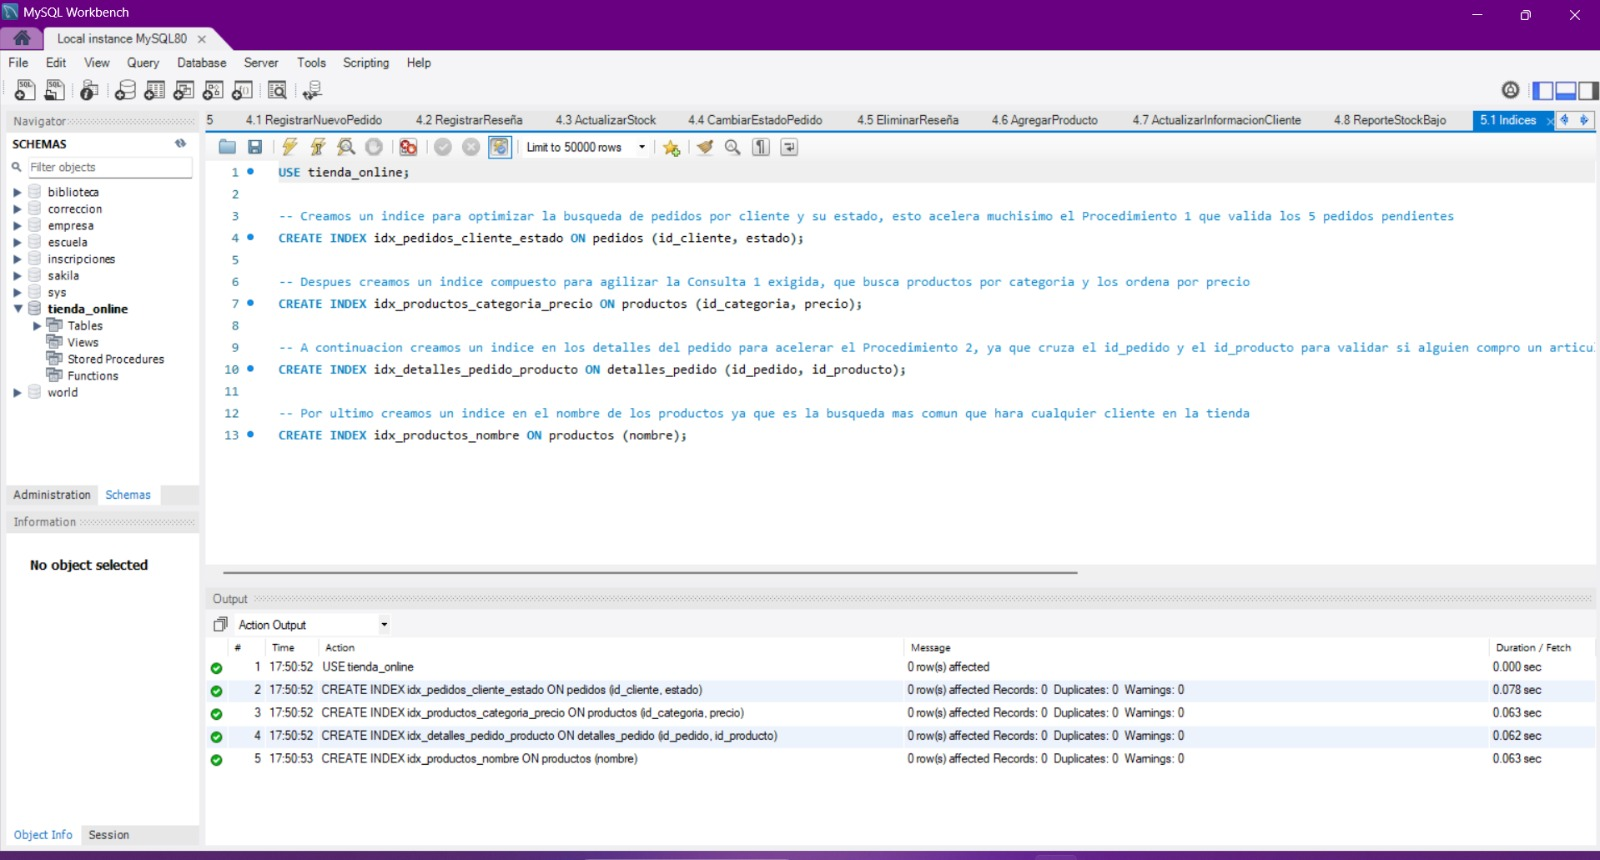
\includegraphics[width=0.9\textwidth]{INDICES.jpeg}
    \caption{Indices creados con exito.}
\end{figure}

\subsection{Análisis EXPLAIN}
\begin{lstlisting}
-- Impacto en la validacion de pedidos pendientes
EXPLAIN SELECT COUNT(*) FROM pedidos WHERE id_cliente = 1 AND estado = 'pendiente';
-- Impacto en la validacion de pedidos pendientes
EXPLAIN SELECT COUNT(*) FROM pedidos WHERE id_cliente = 1 AND estado = 'pendiente';
\end{lstlisting}
Al analizar las consultas con la instrucción \texttt{EXPLAIN}, se demuestra un cambio favorable en el plan de ejecución. El motor utiliza la estructura de árbol del índice (\textit{Using index}) para acceder a los registros solicitados, reduciendo el costo transaccional.

\begin{figure}[H]
    \centering
    \begin{subfigure}{0.48\textwidth}
        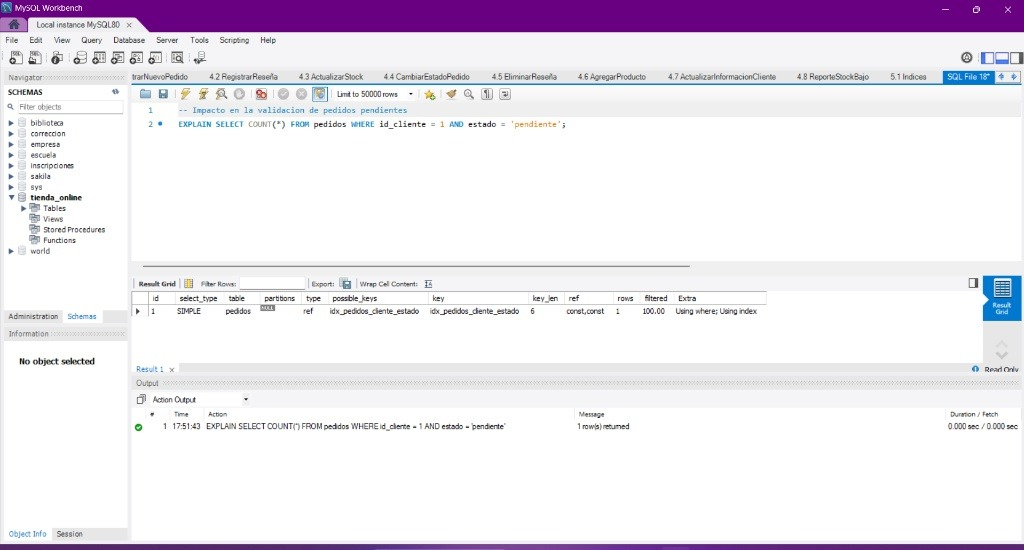
\includegraphics[width=\textwidth]{EX1.jpeg}
        \caption{Impacto en pedidos}
    \end{subfigure}
    \hfill
    \begin{subfigure}{0.48\textwidth}
        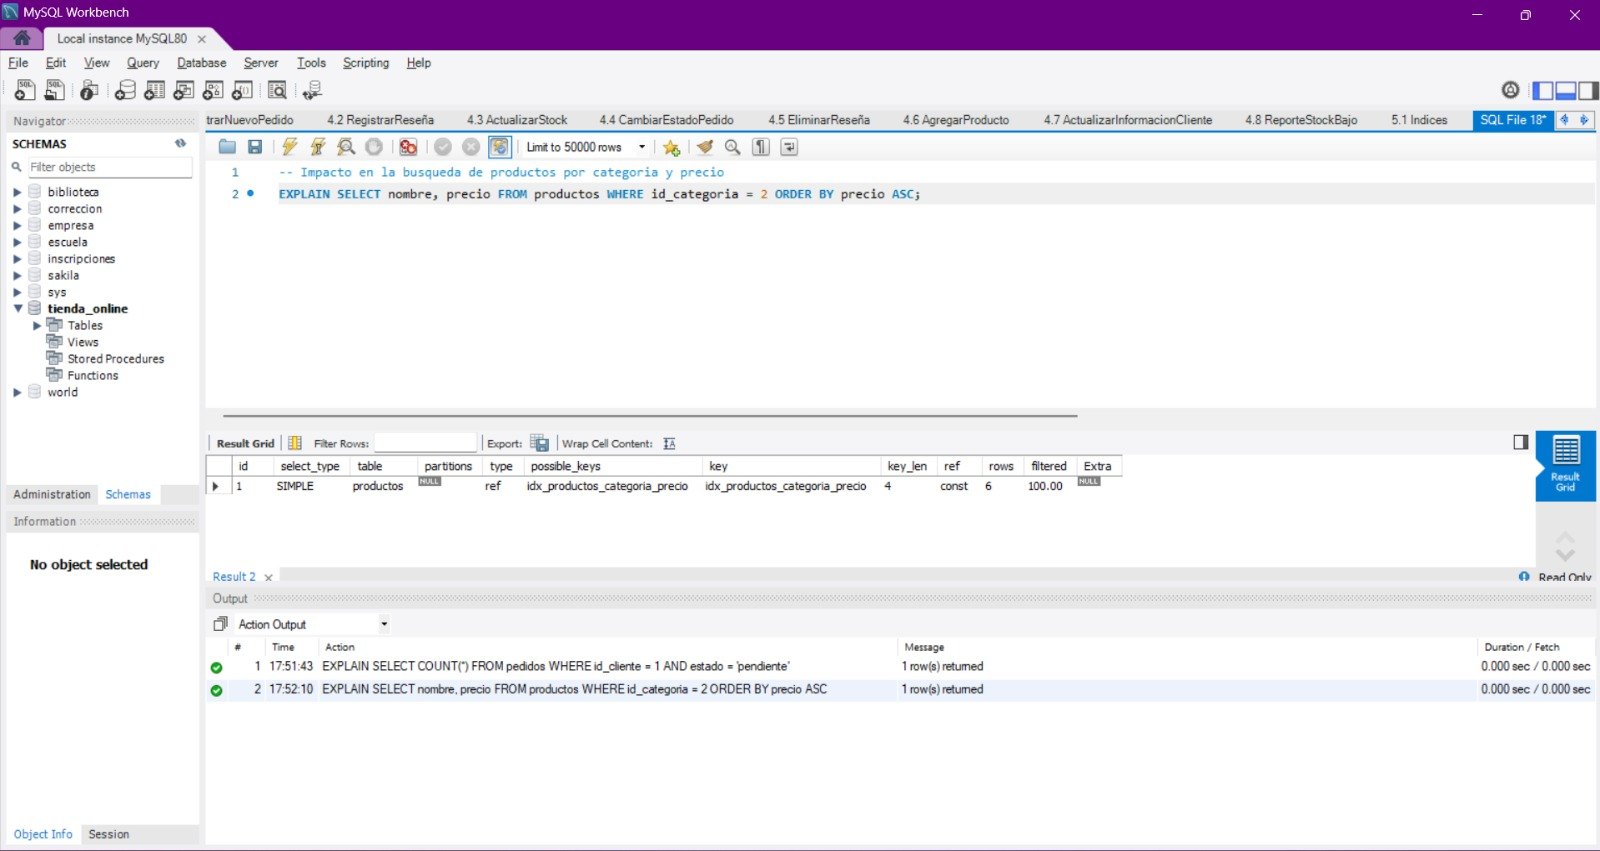
\includegraphics[width=\textwidth]{EX2.jpeg}
        \caption{Impacto en productos}
    \end{subfigure}
\end{figure}

\subsection{Propuestas de Mejoras}
A futuro, el sistema podría beneficiarse de las siguientes optimizaciones:
\begin{itemize}
    \item \textbf{Auditoría mediante Triggers:} Implementar tablas de bitácora pobladas automáticamente por triggers para rastrear cambios importantes, como modificaciones de precios.
    \item \textbf{Particionamiento de Tablas:} En un escenario de alto volumen de intercambio de informacon, particionar la tabla de pedidos por fecha agilizaría los reportes históricos.
\end{itemize}


\section{Conclusiones}
Para la construcción de este sistema, al igual que para cualquier proyecto en el ámbito laboral, es vital dedicar la mayor parte del tiempo a un buen análisis y diseño (en papel). Hacerlo nos facilita enormemente el trabajo de programación y nos evita tener que rediseñar la base de datos una y otra vez.

Si ejecutamos correctamente esta primera fase de análisis, logramos un sistema con pocos o nulos fallos. Y si estos llegan a presentarse, se pueden solucionar con facilidad ajustando ligeramente el código, sin tener que llegar al extremo de una reestructuración total del sistema.

Además, un buen diseño desde la base nos permite garantizar la escalabilidad a futuro, demostrando un verdadero dominio y conocimiento de lo que estamos haciendo. Por ello, planear bien las tablas, los procedimientos almacenados y los índices para agilizar las búsquedas frecuentes es lo que realmente hace que el sistema sea eficiente, robusto y completamente funcional.

\section{Link al repositorio de GitHub}
Enlace al repositorio de GitHub con los scripts físicos del proyecto:
\url{https://github.com/Alexandra075/PROYECTO-FINAL}

\end{document}